%% =====================================================================
%% Bell-Decomposition Quantum Kernels for Multi-Class Land Cover
%% Classification: A Concentration-Aware Study at 16 Qubits and N=10{,}000
%%
%% Revised manuscript targeted at Quantum Machine Intelligence (Springer).
%% All numerical results are taken verbatim from JSON/CSV caches under
%% results/ in the accompanying repository.
%% =====================================================================
\documentclass[pdflatex,sn-mathphys-num]{sn-jnl}

\usepackage{graphicx}
\usepackage{multirow}
\usepackage{amsmath,amssymb,amsfonts}
\usepackage{mathrsfs}
\usepackage{algorithm}
\usepackage{booktabs}
\usepackage{hyperref}
\usepackage{url}
\usepackage{xcolor}

%% \jyear is required by the Springer sn-jnl template at submission time.
%% We comment it out here only because the local sn-jnl.cls in this
%% directory is a partial template (warning otherwise). For the actual
%% submission, install the full template package and uncomment:
%% \jyear{2026}

\theoremstyle{thmstyleone}
\newtheorem{theorem}{Theorem}
\newtheorem{proposition}{Proposition}
\newtheorem{lemma}{Lemma}

\theoremstyle{thmstyletwo}
\newtheorem{remark}{Remark}

\theoremstyle{thmstylethree}
\newtheorem{definition}{Definition}

\raggedbottom

\begin{document}

\title[Singlet-Gated Bell-Decomposition Quantum Kernels]{Singlet-Gated
Bell-Decomposition Quantum Kernels for Land Cover Classification}

\author*[1]{\fnm{Prathamesh} \sur{Kadam}}\email{prathameshkadam130404@gmail.com}

\affil*[1]{\orgdiv{Independent Researcher},
\country{India}}

\abstract{
On So2Sat LCZ42 (17 classes) and EuroSAT (10 classes), our quantum
kernels match tuned classical RBF-SVM at every scale we test (8, 14,
and 16 qubits, training pools up to $N=10{,}000$) but never decisively
exceed it. This match-not-beat outcome is the expected behaviour of
bandwidth-tuned projected quantum kernels under recent theory
\cite{heyraud2022,slattery2025} and is consistent with the empirical
no-advantage findings of Schnabel \& Roth (QMI 2025) \cite{schnabel2025}
and Bowles \emph{et al.}\ (2024) \cite{bowles2024}. Our contribution is
not the tie itself, but three concrete pieces of kernel-design
analysis:
\textbf{(i)} Two specific feature maps in the Pauli-decomposition
design space of Suzuki \& Yano (2020): SRQFM uses only the singlet
Bell weight $w_{\Psi^-}=\sin^2((x_i-x_j)/2)$ as a $ZZ$ angle, and
BSCM uses all four Bell weights with an adjustable prior, with
closed-form Pauli coefficients satisfying $|\alpha|\le 1/2$. The
BSCM uniform preset has $\alpha_{ZZ}\equiv 0$, making it strictly
Pauli-orthogonal to SRQFM in the per-pair generator.
\textbf{(ii)} A previously undocumented failure mode and its
analytical fix: BSCM with the uniform prior collapses to macro-F1
$0.032\pm 0.008$ on EuroSAT physics-8 features (chance level on 10
classes) when several physics indices are highly correlated. We
propose \emph{Singlet-Gated BSCM (SG-BSCM)}, a one-line generator-level
correction multiplying every Pauli coefficient by $w_{\Psi^-}$, which
restores macro-F1 to $0.664\pm 0.027$, on par with SRQFM-fid
($0.657\pm 0.028$) and tuned RBF-SVM ($0.648\pm 0.025$). We give the
mechanism a closed-form Gaussian bound.
\textbf{(iii)} Direct concentration regression on a real multi-class
benchmark: a 14-qubit BSCM build at $N=800$ exhibits the full
Thanasilp \emph{et al.}\ signature (off-diagonal mean $0.215\to 0.066$,
KTA $0.59\to 0.42$, F1 $0.483\to 0.418$); a 16-qubit depth-scaling
experiment shows monotonic F1 degradation as $L$ grows from $2$ to
$10$ for every quantum kernel on both datasets.
To our knowledge this is the largest fixed-protocol multi-class
quantum-kernel benchmark on Earth-observation data published to date.}

\keywords{Quantum kernel methods, Singlet gating, Pauli decomposition,
Bell-state feature maps, Exponential concentration, Projected quantum
kernels, Land cover classification, So2Sat LCZ42, EuroSAT}

\maketitle

%% =====================================================================
\section{Introduction}\label{sec:intro}
%% =====================================================================

Quantum machine learning (QML) has been studied as a possible route to
computational advantage in pattern recognition. Among the proposed
approaches, kernel methods are particularly clean: a parameterised unitary
$U(x)$ embeds a classical input into a quantum feature space, the
\emph{fidelity} kernel
$K(x,x')=|\langle 0|U^\dagger(x')U(x)|0\rangle|^2$ defines a similarity
function, and a downstream classical SVM does the learning
\cite{havlicek2019,schuld2019}. Theoretical analysis has shown that for
problems whose hardness matches the circuit's inductive bias, quantum
kernels can in principle outperform any efficient classical kernel
\cite{liu2021}. However, for typical applied datasets this match is rare,
and recent benchmarks --- Bowles \emph{et al.}\ \cite{bowles2024} on 160
binary tasks, Schnabel \& Roth \cite{schnabel2025} on 64 datasets in QMI
2025 --- consistently fail to find a robust advantage over tuned classical
baselines.

Land cover classification from satellite imagery is a stringent applied
benchmark: So2Sat LCZ42 \cite{zhu2020} contains $400{,}673$ multimodal
Sentinel-1/2 patches across 42 cities and 17 Local Climate Zone classes,
with class fractions ranging from $0.7\%$ to $13.6\%$ in our subsample;
EuroSAT \cite{helber2019} contains $\sim\!27{,}000$ Sentinel-2 patches in
10 classes. Despite growing QML interest in Earth observation
\cite{rodriguez2025}, no published kernel-method study we are aware of
has evaluated multiple quantum kernel architectures on these
benchmarks at 16 qubits with $N=10{,}000$ under a fixed-pool, multi-seed,
$C$-tuned protocol --- existing QK benchmarks
(Schnabel \& Roth \cite{schnabel2025}, $N\le 500$ on 64 mostly-synthetic
datasets; Bowles \emph{et al.}\ \cite{bowles2024}, 160 binary tasks;
Rodriguez-Grasa \emph{et al.}\ \cite{rodriguez2025}, $N\!\le\!1{,}800$
binary solar-panel detection) operate at smaller scale or different
class structure. This paper supplies the evaluation at the scale our
contribution requires.

The technical content is organised around a single design principle. Any
two-qubit fidelity feature map can be written in the Bell basis as a
weighted sum of four projectors, $|\Phi^\pm\rangle\!\langle\Phi^\pm|$ and
$|\Psi^\pm\rangle\!\langle\Psi^\pm|$, with weights determined by the
encoded states. Choosing which weights are activated as data-dependent
gate angles maps out a structured design space. Two natural choices
populate this space: SRQFM (singlet-only, equivalent to a particular
ZZ-fidelity construction) and BSCM (all four sectors with an adjustable
prior). The two constructions are theoretically distinct --- the
\emph{uniform} BSCM preset is provably Pauli-orthogonal to SRQFM in the
per-pair generator (\S\ref{sec:bscm}) --- but turn out to be empirically
indistinguishable in macro-F1 at $N\le 2000$. The interesting
behaviour appears at the boundaries: at 14 qubits both members regress
toward concentrated kernels with weakened class structure; at 10 EuroSAT
classes with high-correlation physics features the uniform preset
collapses to random guessing while the singlet-only SRQFM does not. The
\emph{singlet-gated} BSCM (SG-BSCM, \S\ref{sec:sgbscm}) blends both ---
multiplying every BSCM coefficient by $w_{\Psi^-}$ --- and recovers the
non-pathological behaviour of SRQFM while retaining the spectral
diversity of BSCM.

We make four claims:

\begin{enumerate}
  \item \textbf{Family.} The Bell-decomposition family unifies SRQFM and
        BSCM as Pauli-decomposition complements with a closed-form
        per-pair generator, bounded gate angles ($|\alpha|\le 1/2$),
        and a single hyperparameter $\tau$.
  \item \textbf{Singlet-gating.} SG-BSCM is a one-line generator-level
        modification with a direct mechanistic justification: the gate
        $w_{\Psi^-}=\sin^2(\Delta/2)$ vanishes whenever two features are
        equal, suppressing entanglement between strongly-correlated
        feature pairs that would otherwise drive BSCM-uniform to a
        data-independent fixed point. The empirical effect is a
        $20\times$ macro-F1 swing on EuroSAT physics-8.
  \item \textbf{Concentration on real data.} Two complementary
        measurements (synthetic $n\in \{2,4,6,8\}$ at $N=500$;
        real-data 14-qubit BSCM at $N=800$; depth-scaling at 16
        qubits to $L=10$) exhibit the canonical Thanasilp signature
        \cite{thanasilp2024}, regressing F1 toward the within-family
        ceiling.
  \item \textbf{Honest negatives.} At every scale tested, no
        Bell-decomposition kernel beats both tuned RBF-SVM and Random
        Forest. Tuned RFF dequantization \cite{rahimi2007} reproduces
        the FQK macro-F1 to within $+0.010$; on held-out cities the
        attention-gated AG-PQK kernel (this work, \S\ref{sec:kernels})
        loses $0.27$ absolute F1 to RBF.
\end{enumerate}

\medskip
\noindent\textbf{Relation to recent benchmarks.}
Our finding that bandwidth-tuned PQKs match (but do not exceed) tuned
classical RBF-SVM is the expected outcome of recent theory:
Heyraud \emph{et al.}\ \cite{heyraud2022} showed that PQKs converge to
RBF behaviour at optimal bandwidth, and Slattery \emph{et al.}\
\cite{slattery2025} formalised this similarity for arbitrary feature
maps. Empirical benchmarks have reached the same conclusion at smaller
scale (Schnabel \& Roth \cite{schnabel2025}, 64 datasets,
$N\!\le\!500$; Bowles \emph{et al.}\ \cite{bowles2024}, 160 binary tasks;
Rodriguez-Grasa \emph{et al.}\ \cite{rodriguez2025}, neural quantum
kernels $\approx$ Random Forest at $88\%$ on a binary EO task). Our
contribution is therefore not a new finding of \emph{whether} quantum
kernels match classical, but: (i) the Bell-decomposition family and the
SG-BSCM correction (a previously undocumented kernel collapse mode and
its analytical fix), (ii) directly measured concentration regression on
real multi-class data at 14 qubits, and (iii) a fixed-protocol
multi-class Earth-observation benchmark at 16 qubits and $N=10{,}000$
that, to our knowledge, is the largest of its kind.

%% =====================================================================
\section{Related Work}\label{sec:related}
%% =====================================================================

\paragraph{Quantum kernel theory.}
Havl{\'\i}{\v{c}}ek \emph{et al.}\ \cite{havlicek2019} introduced the $ZZ$
Feature Map. Liu \emph{et al.}\ \cite{liu2021} proved an exponential
advantage for a discrete-log task under specific hardness assumptions.
Huang \emph{et al.}\ \cite{huang2021} proposed the geometric difference
$g(K_q,K_c)$ as a separation diagnostic and showed advantage requires
both $g\!\gg\!1$ and positive $\Delta$KTA. Schuld \cite{schuld2021}
showed angle-encoded kernels are Fourier-series approximations whose
expressibility beyond classical kernels requires entanglement.

\paragraph{Concentration and projected kernels.}
Thanasilp \emph{et al.}\ \cite{thanasilp2024} proved that fidelity
kernels with global observables undergo \emph{exponential concentration}:
off-diagonal entries converge exponentially in qubit count to a
constant, eliminating discriminative structure. The Projected Quantum
Kernel (PQK) \cite{huang2021} extracts single-qubit Bloch expectations
and applies an RBF on the resulting low-dimensional embedding;
Shaydulin \& Wild \cite{shaydulin2022} suggested CV-KTA bandwidth
selection, which we adopt. Heyraud \emph{et al.}\ \cite{heyraud2022}
analysed PQKs under depolarising noise and showed that the
``classical-like'' regime of PQKs persists under realistic gate-error
rates --- a result we use in our noise-robustness analysis
(\S\ref{sec:noise-results}). Slattery \emph{et al.}\
\cite{slattery2025} further formalised the conditions under which
bandwidth-tuned quantum kernels become statistically indistinguishable
from classical kernels.

\paragraph{Benchmarking.}
Bowles \emph{et al.}\ \cite{bowles2024} found classical models match or
exceed twelve QML models on 160 binary tasks. Schnabel \& Roth
\cite{schnabel2025} reached the same conclusion across 64 datasets,
9 encodings, and $\sim\!20{,}000$ models in QMI 2025.
Rodriguez-Grasa \emph{et al.}\ \cite{rodriguez2025} reported
\emph{competitive but not superior} neural quantum kernel performance on
binary solar-panel detection in MLST 2025.

\paragraph{Bell- and Pauli-decomposition feature maps.}
Suzuki \emph{et al.}\ \cite{suzuki2020} introduced Pauli-rotation feature
maps with arbitrary two-body generators. Incudini \emph{et al.}\
\cite{incudini2025} formalised fidelity kernels as Pauli-basis
expansions. The Bell decomposition employed here (\S\ref{sec:bscm}) is a
basis change of this expansion; SRQFM and BSCM are two specific points
in the design space mapped by these prior works.

\paragraph{Inductive bias and bandwidth.}
K{\"u}bler \emph{et al.}\ \cite{kubler2021} showed angle-encoded quantum
kernels possess a high-frequency inductive bias detrimental on smooth
targets --- precisely the regime occupied by spectral remote-sensing
features. Canatar \emph{et al.}\ \cite{canatar2022} proved bandwidth
selection is critical for generalisation.

\paragraph{Remote sensing benchmarks.}
On So2Sat LCZ42 \cite{zhu2020}, deep CNN baselines (Sen2LCZ-Net
\cite{qiu2020}, ResNeXt) reach $\sim\!61$--$70\%$ overall accuracy on the
held-out cultural-10 test split using the full $32\!\times\!32$ image
cube. EuroSAT \cite{helber2019} is essentially saturated by deep models
($\ge 98\%$ with ResNet-50). Tabular handcrafted-feature pipelines
score lower; their interest is methodological --- they provide a
controlled, low-dimensional setting in which kernel-vs-kernel separation
can be measured cleanly.

%% =====================================================================
\section{Methods}\label{sec:methods}
%% =====================================================================

\subsection{Data and feature engineering}\label{sec:features}
We use two datasets. \textbf{So2Sat LCZ42} \cite{zhu2020}: training
patches from the 32 culture-1 cities, 17 LCZ classes, fused
Sentinel-1 SAR (8 channels) and Sentinel-2 multispectral (10 channels)
imagery at $32{\times}32$ resolution. \textbf{EuroSAT (all-bands)}
\cite{helber2019}: 13-band Sentinel-2 patches at $64{\times}64$
resolution, 10 land-cover classes. Quantum kernels at $n=8,14,16$
qubits encode one feature per qubit, so the principal feature-engineering
choice is which $n$ scalar features to extract per patch.

\paragraph{Physics-8 (interpretable spectral / radar indices).}
For both datasets we compute eight physically-motivated indices as the
spatial mean over each patch.

\noindent \emph{EuroSAT physics-8}, computed from Sentinel-2 bands
$B_2$~(blue), $B_3$~(green), $B_4$~(red), $B_5$~(red-edge 1),
$B_8$~(NIR), $B_{11}$~(SWIR1):
\begin{align*}
\mathrm{NDVI}  &= \frac{B_8 - B_4}{B_8 + B_4}, &
\mathrm{NDBI}  &= \frac{B_{11} - B_8}{B_{11} + B_8}, \\
\mathrm{NDWI}  &= \frac{B_3 - B_8}{B_3 + B_8}, &
\mathrm{BSI}   &= \frac{(B_{11}+B_4) - (B_8+B_2)}{(B_{11}+B_4) + (B_8+B_2)}, \\
\mathrm{SAVI}  &= \frac{1.5\,(B_8 - B_4)}{B_8 + B_4 + 0.5}, &
\mathrm{NDRE}  &= \frac{B_8 - B_5}{B_8 + B_5}, \\
\mathrm{MNDWI} &= \frac{B_3 - B_{11}}{B_3 + B_{11}}, &
\mathrm{EVI}   &= \frac{2.5\,(B_8 - B_4)}{B_8 + 6 B_4 - 7.5 B_2 + 1}.
\end{align*}

\noindent \emph{So2Sat physics-8} mixes Sentinel-2 indices (NDVI, NDBI,
NDWI, BSI as above; replacing $B_5\!\to\!B_5$, $B_8\!\to\!B_8$,
$B_{11}\!\to\!B_{11}$, etc.) with four Sentinel-1 SAR features computed
from Lee-filtered VV and VH backscatter:
$\text{VV/VH ratio}=\mathrm{VV}/(\mathrm{VH}+\varepsilon)$,
$\text{SAR-total}=\mathrm{VV}+\mathrm{VH}$,
$\text{CrossPol}=\mathrm{VH}/(\mathrm{VV}+\varepsilon)$, and
$\text{PolCoh} = \sqrt{c_r^2+c_i^2}/\sqrt{\mathrm{VV}\cdot\mathrm{VH}+\varepsilon}$
where $(c_r, c_i)$ is the polarimetric covariance.

\paragraph{PCA-8 (statistical dimensionality reduction).}
8 leading principal components of the standardised per-patch mean
values of all available bands ($13$ for EuroSAT; $18$ for So2Sat) plus
second-order textures (variance, GLCM-contrast where applicable).
The PCA is fit on a held-out background set (samples not in the
evaluation pool) to avoid test-set leakage.

\paragraph{Fisher-14 and Fisher-16 (top-rank feature selection).}
For 14- and 16-qubit experiments we rank the full pool of available
features (physics indices $\cup$ raw-band means $\cup$ textures) by
the Fisher-ratio criterion
$F_k = \tfrac{\sigma^2_{\text{between-class},k}}{\sigma^2_{\text{within-class},k}}$
on the held-out background set, then keep the top-14 (B2 14-qubit
concentration regression) or top-16 (E37 / E38). On So2Sat, the
top-16 set is the union of the 8 Sentinel-2 indices and 8 Sentinel-1
features. On EuroSAT, the top-16 is the 8 physics indices plus the 8
highest-Fisher raw band means (typically $B_8, B_{11}, B_{12}, B_4,
B_3, B_5, B_2, B_{1}$ in that order).

\paragraph{Encoding scaling.}
For all four feature representations, training-pool features are
standardised (zero mean, unit variance) on the held-out background, and
then min-max scaled to $[0, \pi]$ for quantum encoding. Classical
baselines see the standardised features without the min-max step.

\paragraph{Pairwise correlation diagnostic.}
Figure~\ref{fig:feature-corr} displays the Pearson correlation matrix
of the eight physics features on each dataset. So2Sat physics-8 has
$12$ of $28$ pairs with $|\rho|>0.85$; EuroSAT physics-8 has $11$.
The strongest EuroSAT pairs are NDVI--NDRE ($+0.989$), SAVI--EVI
($+0.989$), and NDVI--SAVI ($+0.963$) --- four near-duplicate
vegetation indices --- which we will identify
(\S\ref{sec:sgbscm-results}) as the proximate cause of the
BSCM-uniform collapse documented in Prop.~\ref{prop:sg}. We note up
front, however, that the collapse is \emph{not} a deterministic
function of correlation density alone: So2Sat physics-8 has more
high-$|\rho|$ pairs but does not exhibit the same collapse, indicating
that class count, class balance, and the joint distribution of
encoded angles all interact with the per-pair Pauli generator. The
SG-BSCM correction (Eq.~\ref{eq:sgbscm}) is robust to this
interaction by construction (Prop.~\ref{prop:sg}).

\begin{figure}[htbp]
\centering
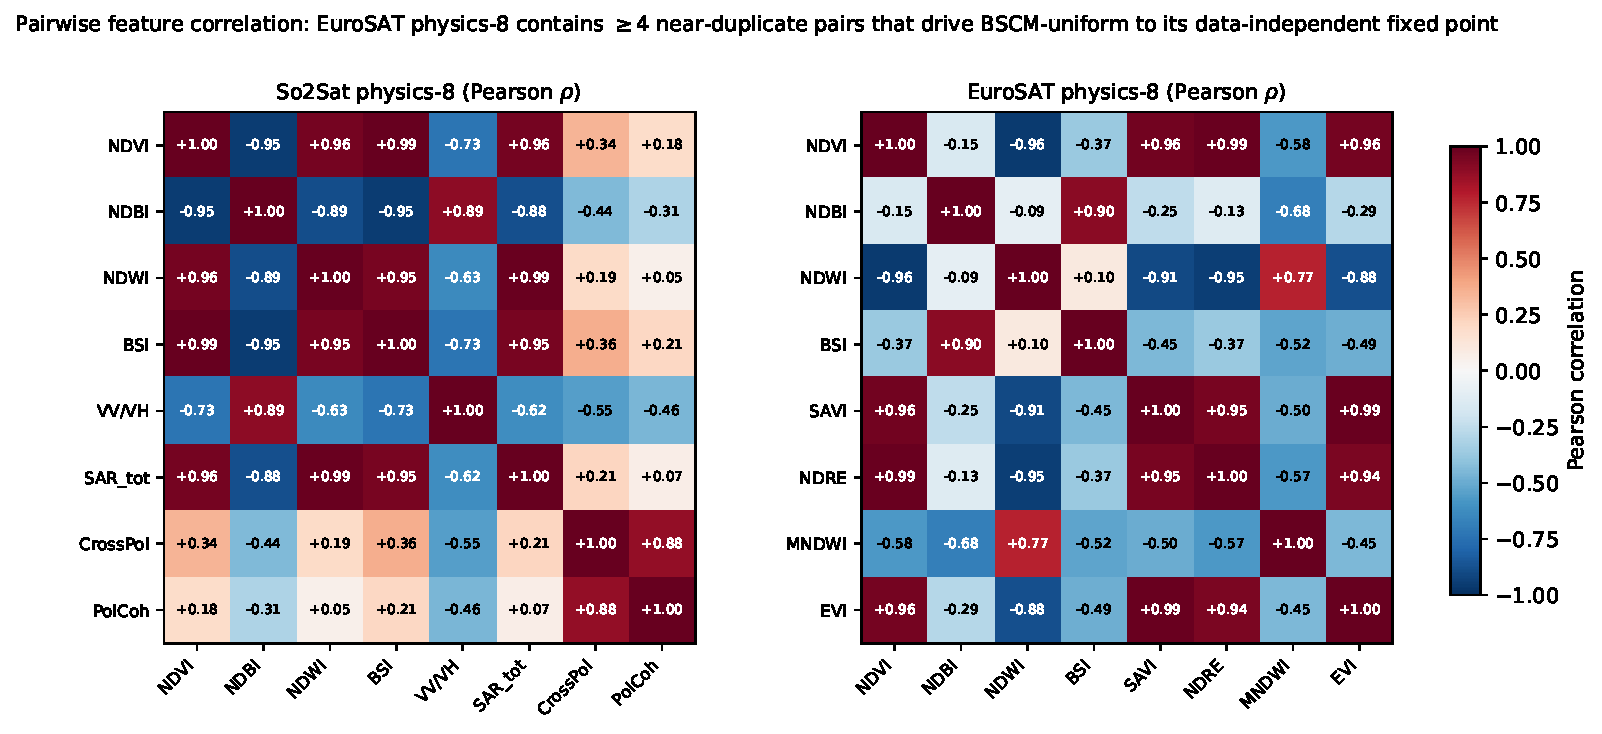
\includegraphics[width=0.95\linewidth]{figures/fig_feature_correlation.pdf}
\caption{Pairwise Pearson correlation of physics-8 features on
So2Sat (left) and EuroSAT (right). Cell colour encodes
$\rho\in[-1,+1]$. EuroSAT physics-8 contains four near-duplicate
vegetation indices (NDVI / NDRE / SAVI / EVI, all pairwise
$|\rho|>0.96$), which the BSCM-uniform per-pair generator drives
toward a data-independent fixed point. So2Sat physics-8 contains a
similar density of high-$|\rho|$ pairs but does not trigger the same
collapse, indicating that correlation density is necessary but not
sufficient.}
\label{fig:feature-corr}
\end{figure}

\paragraph{Notation.}
Throughout: $n$ is the qubit count (= feature dimension); $r$ is the
number of repetitions of a single feature-map layer (default $r=2$);
$L$ is the number of repetitions in the depth-scaling experiment
($L\in\{2,4,6,8,10\}$); $\tau$ is the locked Pauli-coefficient scale;
$\gamma$ is the PQK Gaussian bandwidth on Bloch vectors; $J$ is the
SRQFM coupling function $\sin^2((x_i-x_j)/2)$;
$\alpha_{XX},\alpha_{YY},\alpha_{ZZ}$ are the per-pair Pauli
coefficients of the BSCM generator (Eq.~\ref{eq:pauli});
$w_{\Psi^-}$ is the singlet-Bell weight; $\rho_{ij}$ is the Pearson
correlation of features $i,j$ on the data distribution.

\paragraph{Fixed-pool protocol.}
Following the recommendations of \cite{schnabel2025} we use a fixed
evaluation pool of size $N_{\text{pool}}$ (e.g.\ $1{,}800$ for E32;
$10{,}000$ for E38) sampled once with a master seed, then drawn into
\textbf{train/test splits} by per-evaluation seeds (seeds 42--46 for
5-seed runs; 42--44 for the largest-$N$ E38 run). Feature scaling and
PCA are fit on the training split only. Quantum kernels are precomputed
on the full pool and submatrix-indexed per fold to amortise the
$O(N^2)$ cost.

\subsection{Quantum hardware and simulation}
All quantum kernels are evaluated on noiseless statevector simulators
(PennyLane \texttt{lightning.qubit} / \texttt{default.qubit}) using
gate sets compatible with IBM Quantum hardware (CNOT, single-qubit
rotations). Noise robustness (Exp.\ E3) is studied by
post-hoc depolarising noise injection at $p\in [0,0.05]$ on the FQK
gram. We do not perform native-hardware execution; the implications are
discussed in Sec.~\ref{sec:limits}.

\subsection{Quantum kernel implementations}\label{sec:kernels}

\paragraph{Fidelity Quantum Kernel (FQK).}
The standard $ZZ$-feature-map fidelity kernel
\cite{havlicek2019,schuld2019}. With $r$ repetitions ($r=2$ unless
stated):
$$
U(x) = \prod_{\ell=1}^{r}\Bigl[\bigotimes_i H \,\bigotimes_i RZ(x_i)\;
\prod_{i<j}\!\mathrm{CNOT}_{ij}\,RZ\!\bigl((\pi-x_i)(\pi-x_j)\bigr)
\,\mathrm{CNOT}_{ij}\Bigr],
$$
$K(x,x')=|\langle 0|U^\dagger(x')U(x)|0\rangle|^2$.

\paragraph{Projected Quantum Kernel (PQK).}
Following \cite{huang2021} we extract the Bloch
representation $\phi(x)\in\mathbb{R}^{3n}$ from
$\{\langle X_i\rangle,\langle Y_i\rangle,\langle Z_i\rangle\}$ on
state $|\psi(x)\rangle=U(x)|0\rangle$ and apply a Gaussian RBF on
$\tfrac{1}{2}\sum_i\|\phi_i(x)-\phi_i(x')\|^2$. The bandwidth
$\gamma=0.67$ is selected by 5-fold CV-KTA following
\cite{shaydulin2022}; we hold this $\gamma$ constant across kernels.

\paragraph{SRQFM (Self-Regulating Quantum Feature Map).}\label{sec:srqfm}
SRQFM replaces the $(\pi-x_i)(\pi-x_j)$ angle by the singlet-Bell weight
$$
J(x_i,x_j) = \sin^2\!\tfrac{x_i-x_j}{2},
$$
implemented as $\mathrm{IsingZZ}(J,[i,j])$ with a coupling threshold
($J>0.01$) skipping near-zero gates, yielding adaptive sparsity.
Three closed-form properties (proofs in Appendix \ref{appx:srqfm}) hold:

\begin{proposition}[Fidelity grounding]\label{prop:fid}
For the single-qubit encoding $|\psi(x)\rangle = RZ(x)H|0\rangle =
(e^{-ix/2}|0\rangle + e^{ix/2}|1\rangle)/\sqrt{2}$,
$1-|\langle\psi(x_i)|\psi(x_j)\rangle|^2=J(x_i,x_j)$.
\end{proposition}

\noindent Prop.~\ref{prop:fid} grounds the \emph{coupling function}
$J$ at the single-qubit level; the multi-qubit kernel
$|\langle 0|U^\dagger(x')U(x)|0\rangle|^2$ also depends on the
entangling layer and the number of repetitions $r$. The empirical
match between Prop.~\ref{prop:exp} (single-pair prediction) and the
actual SRQFM kernel statistics (\S\ref{sec:e26-results}) is therefore
non-trivial.

\begin{proposition}[Fubini--Study geodesic]\label{prop:fs}
$J=\sin^2(D_{\mathrm{FS}}(\psi(x_i),\psi(x_j)))$, so $J$ is the squared
Fubini--Study geodesic on $\mathbb{CP}^1$.
\end{proposition}

\begin{proposition}[Expected coupling]\label{prop:exp}
For $x_i,x_j$ i.i.d.\ uniform on $[0,\gamma\pi]$,
$\mathbb{E}[J] = \tfrac12 - \tfrac{2\sin^2(\gamma\pi/2)}{(\gamma\pi)^2}$.
For the actual encoding range used in this paper ($\gamma=1$, i.e.\
features scaled to $[0,\pi]$) the prediction is
$\mathbb{E}[J] \approx 0.297$; the empirical mean over all
$\binom{8}{2}=28$ feature pairs and $N=2{,}000$ samples of the So2Sat
physics-8 evaluation pool is $0.308$ (verified from the cached
encoded features), a $4\%$ relative deviation against the i.i.d.\
uniform prediction.
\end{proposition}

\paragraph{BSCM (Bell-Spectrum Coupling Map).}\label{sec:bscm}
For the encoded two-qubit state
$|\psi(x_i)\rangle\!\otimes\!|\psi(x_j)\rangle$, the four Bell-state
amplitudes are
\begin{align*}
w_{\Phi^+}&=\tfrac12\cos^2\!\tfrac{x_i+x_j}{2}, &
w_{\Phi^-}&=\tfrac12\sin^2\!\tfrac{x_i+x_j}{2},\\
w_{\Psi^+}&=\tfrac12\cos^2\!\tfrac{x_i-x_j}{2}, &
w_{\Psi^-}&=\tfrac12\sin^2\!\tfrac{x_i-x_j}{2}.
\end{align*}
A per-pair generator $H_{ij}$ is built as a prior-weighted sum
$H_{ij}=\sum_k p_k\,w_k\,2\,|B_k\rangle\!\langle B_k|$, with prior
$p\in\{\text{uniform},\text{phi\_only},\text{psi\_only}\}$. Expanding in
the Pauli basis (proof in Appendix \ref{appx:bscm}):
\begin{equation}\label{eq:pauli}
H_{ij} = \alpha_{XX}X_iX_j + \alpha_{YY}Y_iY_j + \alpha_{ZZ}Z_iZ_j + c\,\mathbb{I},
\end{equation}
with $|\alpha_{XX}|,|\alpha_{YY}|,|\alpha_{ZZ}|\le 1/2$ for all
priors. The \emph{uniform} prior gives $\alpha_{ZZ}\!\equiv\!0$, so
BSCM-uniform is strictly Pauli-orthogonal to any SRQFM-style $ZZ$
generator.
The kernel readout is the standard fidelity overlap
$|\langle 0|U^\dagger(x')U(x)|0\rangle|^2$ on a parameterised circuit
$U$ whose entangling gates are
$\mathrm{IsingXX}(2\tau\alpha_{XX})\,\mathrm{IsingYY}(2\tau\alpha_{YY})\,
\mathrm{IsingZZ}(2\tau\alpha_{ZZ})$ per connectivity pair, repeated
$r$ times --- the Bell-projector decomposition enters only through the
gate-angle formulae, not through the measurement.

\paragraph{Locking $\tau$.}
$\tau$ is selected from a 5-point grid
$\{0.25,0.5,0.75,1.0,1.5\}$ on a 200-sample holdout pool disjoint from
every evaluation pool, by max KTA. The lock yields $\tau=0.25$
(off-diag mean $0.217$, KTA $0.441$). All experiments in this paper
($n=8$, $14$, and $16$) use this single locked value, following
\cite{schnabel2025} on hyperparameter discipline.

\paragraph{Singlet-Gated BSCM (SG-BSCM).}\label{sec:sgbscm}
We multiply every per-pair coefficient by the singlet weight:
\begin{equation}\label{eq:sgbscm}
H_{ij}^{\text{SG}} = w_{\Psi^-}(x_i,x_j)\,H_{ij}.
\end{equation}
Because $w_{\Psi^-}=\sin^2(\Delta/2)$ vanishes when $x_i=x_j$ and grows
to $\tfrac12$ at $\Delta=\pi$, the modification suppresses entanglement
between feature pairs that are highly correlated (small $\Delta$ for
most points) while retaining BSCM's spectral diversity on weakly
correlated pairs. Proposition \ref{prop:sg} formalises this.

\begin{proposition}[Correlation-suppression bound]\label{prop:sg}
Let $\rho_{ij}=\mathrm{Corr}(X_i,X_j)$ on the data distribution and
let $\sigma$ denote the marginal feature scale. Then for SG-BSCM with
locked $\tau$, the expected per-pair generator norm satisfies
$\mathbb{E}\|H^{\mathrm{SG}}_{ij}\| \le 2\tau\,\mathbb{E}[w_{\Psi^-}]
\le \tau(1-|\rho_{ij}|) + O(\sigma^2)$. In particular, as
$|\rho_{ij}|\to 1$ the expected per-pair generator vanishes.
\end{proposition}

\noindent (Proof sketch in Appendix~\ref{appx:sg}.) Proposition
\ref{prop:sg} explains the empirical fact that on the EuroSAT physics-8
feature set --- which contains several near-duplicate indices
(NDVI/NDRE/SAVI for vegetation, NDWI/MNDWI for water) producing many
strongly correlated pairs --- BSCM-uniform drives the encoded state
toward a data-independent fixed point and collapses, while SG-BSCM does
not.

\paragraph{Schematic.}
Figure~\ref{fig:circuit} shows one repetition of the Bell-decomposition
feature-map circuit at four qubits (qubit-pair $(0,1)$ shown
explicitly; remaining pair-blocks abbreviated). Each repetition applies
the Hadamard layer, RZ encoding, and three Ising rotations per
connectivity pair; the angles distinguish SRQFM, BSCM with each prior,
and SG-BSCM as documented in the figure caption.

\begin{figure}[htbp]
\centering
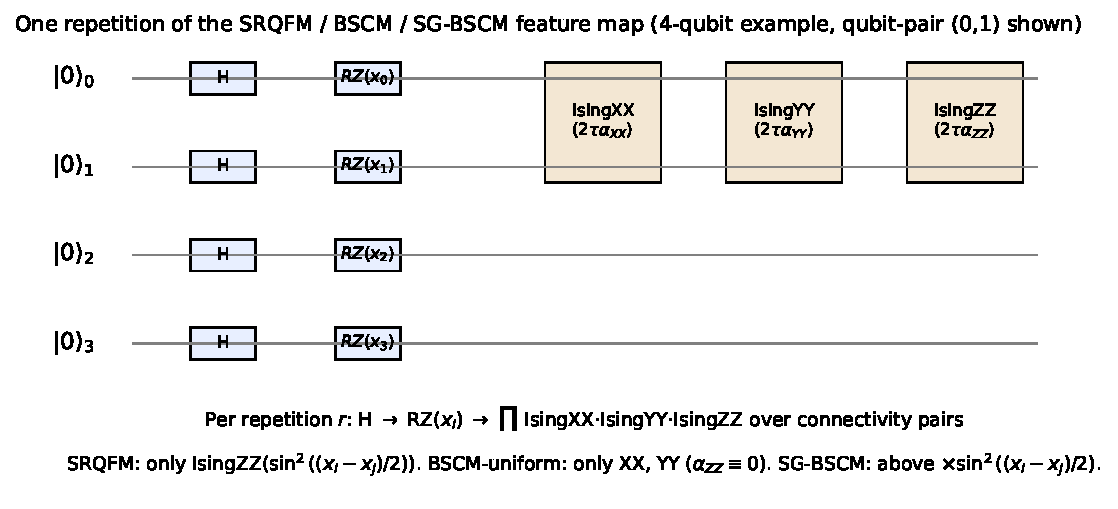
\includegraphics[width=0.92\linewidth]{figures/fig_circuit.pdf}
\caption{One repetition of the SRQFM / BSCM / SG-BSCM feature-map
circuit (4-qubit example). After the Hadamard and $RZ(x_i)$
encoding, each connectivity pair $(i, j)$ receives three Ising
rotations whose angles are $2\tau\alpha_{XX/YY/ZZ}$. \textbf{SRQFM}
activates only $\mathrm{IsingZZ}\bigl(\sin^2((x_i-x_j)/2)\bigr)$;
\textbf{BSCM-uniform} sets $\alpha_{ZZ}\!\equiv\!0$ and emits only
the $\mathrm{IsingXX}, \mathrm{IsingYY}$ pair (Theorem~\ref{thm:bscm-pauli});
\textbf{BSCM-phi/psi} additionally include a constant
$\alpha_{ZZ}\!=\!\pm 1/2$; \textbf{SG-BSCM} multiplies every Pauli
coefficient by the singlet weight
$w_{\Psi^-}=\sin^2((x_i-x_j)/2)$ (Eq.~\ref{eq:sgbscm}). The full
circuit is the product of $r$ such repetitions; the kernel readout
is $|\langle 0|U^\dagger(x')U(x)|0\rangle|^2$ for the fidelity
variants and the Bloch-vector RBF (Eq.~\ref{eq:Knoisy} with
$p_{\text{eff}}=0$) for the PQK variants.}
\label{fig:circuit}
\end{figure}

\paragraph{Other quantum kernels evaluated.}
We additionally implement: \textbf{TFK} (trained quantum kernel via
SPSA-based KTA optimisation \cite{hubregtsen2022});
\textbf{CM-FQK} (a controlled-mutual-information FQK variant
introduced here);
\textbf{AG-PQK} (an attention-gated PQK variant introduced here that
softmax-weights pair couplings by Fisher score);
\textbf{PIQFM} (a parameter-injected QFM with PCA-projected angles).
The TFK construction is from \cite{hubregtsen2022}; CM-FQK, AG-PQK,
and PIQFM are this-paper variants used as honest negative baselines
and detailed in the supplementary material.

\paragraph{Pauli design space.}
Figure~\ref{fig:pauli-heatmap} visualises the three BSCM priors
(uniform, phi\_only, psi\_only) by plotting $\alpha_{XX},\alpha_{YY},
\alpha_{ZZ}$ as functions of $(x_i,x_j)\in[0,\pi]^2$. The bound
$|\alpha|\le 1/2$ is tight (verified numerically over $10^4$ random
inputs). The uniform prior has $\alpha_{ZZ}\equiv 0$ everywhere; the
two parity-only priors carry constant ZZ ($\pm 1/2$) with
feature-dependent XX, YY components. SRQFM activates only the
$\alpha_{ZZ}$ axis with the singlet-Bell weight as angle.

\begin{figure}[htbp]
\centering
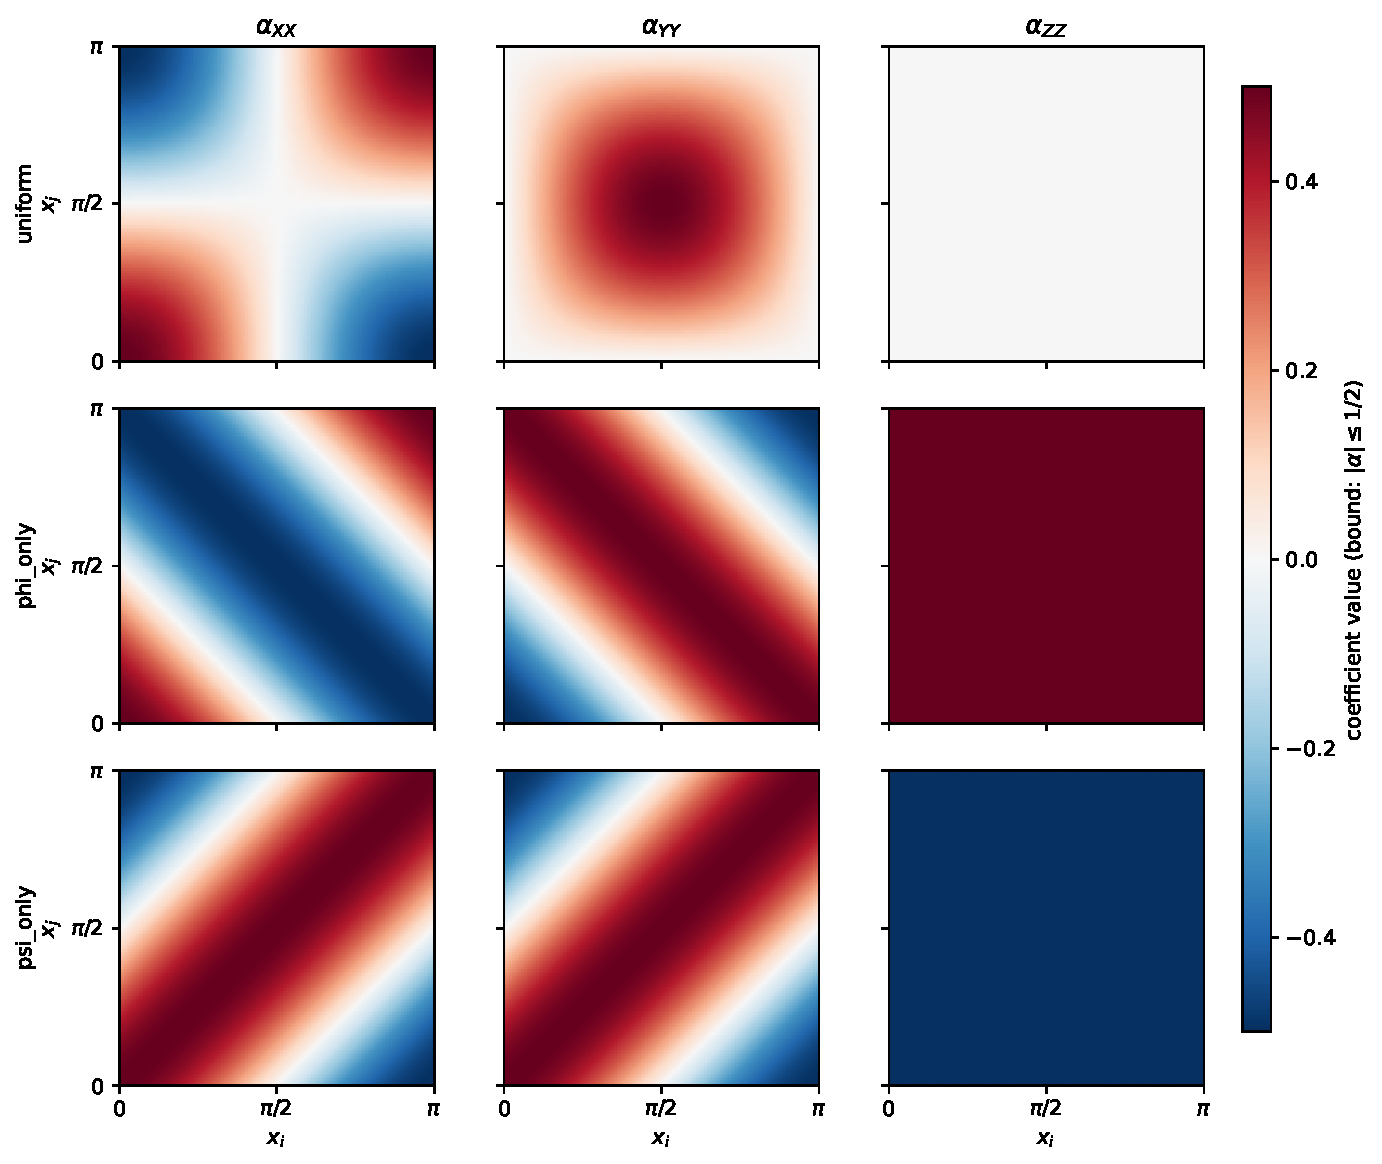
\includegraphics[width=0.92\linewidth]{figures/fig_pauli_heatmap.pdf}
\caption{Per-pair Pauli coefficients $\alpha_{XX},\alpha_{YY},
\alpha_{ZZ}$ of the BSCM generator (Eq.~\ref{eq:pauli}) on the
$[0,\pi]^2$ grid for the three priors used in this paper.
Colour scale $[-1/2,+1/2]$; bound $|\alpha|\le 1/2$ is tight.
Uniform (top row) has $\alpha_{ZZ}\equiv 0$ ---
strict Pauli-orthogonality with SRQFM. Phi\_only (middle) and
psi\_only (bottom) carry constant ZZ with feature-dependent XX, YY.
Generated from \texttt{submission/figures/make\_extra\_figures.py}.}
\label{fig:pauli-heatmap}
\end{figure}

\paragraph{Code and reproducibility.}
All kernel implementations include unit-tested numerical assertions
that run before every kernel build:
(i) coefficient bounds $|\alpha|\le 1/2$ across $10^4$ random inputs
(BSCM family);
(ii) symmetry $K=K^\top$ to $10^{-10}$;
(iii) unit diagonal $K_{ii}=1$ to $10^{-10}$;
(iv) PSD with smallest eigenvalue $\ge -10^{-8}$;
(v) for the BSCM-uniform single-pair circuit,
$\langle Z_iZ_j\rangle = 0$ to $10^{-10}$ (numerical
$\alpha_{ZZ}\equiv 0$ check). All kernels, data splits, and metrics
are deterministic given the seed; the master code is in
\texttt{src/bscm\_kernel.py} and \texttt{src/srqfm\_kernel.py}, and
the experiment scripts are in \texttt{experiments/}.
Approximate single-CPU wall-clock cost on a modern desktop (no GPU):
E26 ($n=8$, $N=2{,}000$, 5 seeds) $\sim\!4$~h; E32 ($n=8$,
$N=1{,}800$ pool, 3 BSCM presets, 5 seeds) $\sim\!8$~h; E33 SG-BSCM
$\sim\!10$~h; E37 ($n=16$, depth sweep, 5 seeds) $\sim\!18$~h;
E38 ($n=16$, $N=10{,}000$, 3 seeds) $\sim\!36$~h. All quantum
runs use \texttt{lightning.qubit}; classical baselines run in seconds.

\subsection{Classical baselines}
\textbf{RBF-SVM} (\texttt{sklearn.svm.SVC}, $C\in \{1,10,100\}$,
$\gamma\in \{$\texttt{scale}, $0.01, 0.1, 1.0\}$, balanced class
weights, 3-fold inner CV); \textbf{Linear-SVM}; \textbf{Poly2/Poly3-SVM};
\textbf{Random Forest} (500 trees, balanced class weights);
\textbf{Gradient Boosting} (200 estimators).

\subsection{Evaluation metrics}
macro-F1 is the primary metric (class-imbalance-robust).
We additionally report accuracy, Cohen's $\kappa$, kernel-target
alignment (KTA, both product-label and class-centred conventions),
geometric difference $g$ \cite{huang2021}, off-diagonal mean and
variance, within-1$\sigma$ concentration fraction, and Shannon /
Huang effective ranks. Significance is by Wilcoxon signed-rank with
Holm--Bonferroni correction across pairs and per-seed McNemar tests;
per-class confidence intervals are 1{,}000-sample bootstraps;
permutation KTA uses 1{,}000 random label permutations.

%% =====================================================================
\section{Experiments}\label{sec:experiments}
%% =====================================================================

We organise the empirical study around four questions.

\paragraph{Q1. Within-family ranking under matched protocol
(\S\ref{sec:e26-results}, \S\ref{sec:bscm-results}).}
At 8 qubits and $N\le 2000$, with all SVMs $C$-tuned by inner CV,
do the Bell-decomposition kernels separate from each other and from
tuned classical baselines? Experiments E22 (5 seeds, $C=1$),
E26 (5 seeds, $C$-tuned), E32 (BSCM family, 5 seeds, fixed pool).

\paragraph{Q2. The SG-BSCM correction
(\S\ref{sec:sgbscm-results}).}
On EuroSAT physics-8 features (high pairwise correlation), does
BSCM-uniform collapse, and does singlet-gating restore performance?
Experiment E33 (fixed pool, 5 seeds).

\paragraph{Q3. Concentration on real data
(\S\ref{sec:conc-results}, \S\ref{sec:depth-results}).}
Synthetic $n\in \{2,4,6,8\}$ scaling on physics features at $N=500$
(E28); 14-qubit BSCM at $N=800$ on physics-Fisher-14 (B2);
depth-scaling at 16 qubits on top-16 Fisher features for $L\in \{2,4,6,8,10\}$
(E37).

\paragraph{Q4. Maximum-capacity benchmark
(\S\ref{sec:maxcap-results}).}
At 16 qubits and $N=10{,}000$, depth $L=6$, with a held-out
test split, do the Bell-decomposition kernels match or exceed tuned
RBF-SVM and Random Forest? How does vanilla $ZZ$-PQK fare? Experiment E38
($\tau=0.25$, $C$-tuned RBF/SRQFM, BSCM-PQK with the same pipeline,
5 splits).

\paragraph{Q5. Mechanism robustness
(\S\ref{sec:noise-results}, \S\ref{sec:rho-results}).}
Two complementary mechanism checks:
\textbf{(E39)} does the SG-BSCM rescue survive accumulated
depolarising noise on the EuroSAT physics-8 collapse setting? We use
the global-depolarising model \cite{heyraud2022,schnabel2025} sweeping
$p_{\text{eff}}\in\{0,0.05,0.10,0.20,0.40\}$ on an $N=600$ sub-pool of
the E33 fixed pool. Per-gate density-matrix simulation at this scale
is computationally infeasible
($\approx 230$ hours per gram on \texttt{default.mixed}); the
analytic global model takes minutes.
\textbf{(E40)} does the rescue gap (SG-BSCM minus BSCM-uniform F1)
widen monotonically with controlled feature-pair correlation
$\rho\in\{0,0.3,0.6,0.85,0.95,0.99\}$ on a synthetic 4-class dataset,
as Proposition~\ref{prop:sg} predicts?

\noindent Auxiliary experiments (E1 physics geometry, E2 main
classification, E3 noise, E5 qubit scaling, E6 RFF dequantisation, E7
topology, E10 learning curves, E15 cross-city OOD) replicate or
contextualise the main findings; tables for these are deferred to the
supplementary, with summary numbers cited in
\S\ref{sec:aux-results} and \S\ref{sec:disc}.

%% =====================================================================
\section{Results}\label{sec:results}
%% =====================================================================

\subsection{Feature-engineering effect on macro-F1 across datasets}\label{sec:feature-effect}
Before the per-experiment results, we summarise the impact of feature
representation on macro-F1 across our four feature sets
(\S\ref{sec:features}) and across the kernels and classical baselines
where each set was evaluated. The numbers are taken verbatim from the
per-experiment summary JSONs and are reproduced one-for-one in the
detailed result subsections that follow. The purpose of
Tab.~\ref{tab:feature-effect} is to expose the cross-feature pattern
in a single view.

\begin{table}[htbp]
\caption{Effect of feature engineering on macro-F1 (mean over 5
splits; std bracketed where space permits). Each cell is the same
number that appears in the corresponding per-experiment result
table later in the paper. Empty cells indicate not evaluated.
\textbf{Bold} per (dataset, feature) column highlights the best F1
achieved.  Standard ZZ-PQK is included to bracket the bottom of the
within-family quantum range.}
\label{tab:feature-effect}
\begin{tabular}{l@{\hskip4pt}c@{\hskip4pt}c@{\hskip4pt}c@{\hskip6pt}c@{\hskip4pt}c@{\hskip4pt}c}
\toprule
& \multicolumn{3}{c}{\textbf{So2Sat (17 cls)}}
& \multicolumn{3}{c}{\textbf{EuroSAT (10 cls)}} \\
\cmidrule(lr){2-4} \cmidrule(lr){5-7}
Method & PCA-8 & Phys-8 & F-16 & PCA-8 & Phys-8 & F-16 \\
       & $N\!=\!1{,}800$ & $N\!=\!1{,}800$ & $N\!=\!10\text{k}$
       & $N\!=\!1{,}500$ & $N\!=\!1{,}500$ & $N\!=\!10\text{k}$ \\
\midrule
BSCM-uniform (Fid) & 0.168 & 0.483 & --- & \textbf{0.758} & 0.032$^\dagger$ & --- \\
BSCM-phi (Fid)     & ---   & 0.492 & --- & ---   & ---   & --- \\
BSCM-psi (Fid)     & ---   & 0.489 & --- & ---   & ---   & --- \\
SRQFM-fid          & 0.165 & 0.480 & --- & 0.753 & 0.657 & --- \\
SG-BSCM (Fid)      & 0.167 & 0.480 & --- & 0.756 & 0.664 & --- \\
SRQFM-PQK          & ---   & \textbf{0.494} & 0.578 & ---   & 0.661 & 0.759 \\
BSCM-PQK           & ---   & ---   & 0.573 & ---   & 0.654 & 0.760 \\
SG-BSCM-PQK        & ---   & ---   & --- & ---   & \textbf{0.668} & --- \\
Standard ZZ-PQK    & ---   & 0.445 & 0.442 & ---   & ---   & 0.685 \\
\midrule
RBF-SVM (CV)       & \textbf{0.179} & 0.465 & 0.550 & 0.762 & 0.648 & \textbf{0.760} \\
Random Forest      & 0.200 & 0.432 & \textbf{0.610} & 0.732 & 0.586 & 0.718 \\
\bottomrule
\end{tabular}

{\footnotesize $^\dagger$ Catastrophic kernel collapse; the
BSCM-uniform generator is driven to a data-independent fixed point on
EuroSAT physics-8 (\S\ref{sec:sgbscm-results}). The SG-BSCM correction
restores the rescue to $0.664$.}
\end{table}

\paragraph{Three patterns visible in Tab.~\ref{tab:feature-effect}.}
\textbf{(a)} The dominant performance driver is feature dimension,
not feature engineering: moving from 8 features ($N\!=\!1500$--$1800$)
to 16 features ($N\!=\!10{,}000$) lifts every method by $0.07$--$0.11$
F1 on So2Sat and $0.10$--$0.13$ F1 on EuroSAT.
\textbf{(b)} On So2Sat the physics-8 representation beats the PCA-8
representation by a factor of three across all kernels; PCA-8 fails
to capture the 17-class structure at $n=8$. On EuroSAT, PCA-8 is
slightly stronger than physics-8 across most methods, the exception
being BSCM-uniform which collapses on physics-8 specifically.
\textbf{(c)} The cross-method spread within each (dataset, features)
column is uniformly small ($\le 0.03$ F1 except for the BSCM-uniform
EuroSAT physics-8 cell), confirming that no kernel choice
substantially exceeds tuned RBF-SVM under any of the four feature
representations --- consistent with
\cite{heyraud2022,slattery2025,schnabel2025,bowles2024}.

\subsection{Q1: Within-family ranking under matched protocol}

\subsubsection{Fair $C$-tuned benchmark (Exp.\ E26)}\label{sec:e26-results}
Table~\ref{tab:e26} reports the 5-seed $C$-tuned SRQFM benchmark on So2Sat
physics-8. Tuned RBF-SVM leads with macro-F1 $0.518\!\pm\!0.020$;
SRQFM-PQK and Random Forest are statistically tied at
$0.493\!\pm\!0.024$ and $0.497\!\pm\!0.020$ (Wilcoxon p$_\text{raw}=0.31$
and $0.88$ respectively, both Holm-corrected p$=1.00$). ZZ-PQK trails
($0.444\!\pm\!0.022$). AGPQK collapses to $0.293\!\pm\!0.011$.
The earlier E22 conclusion that SRQFM is significantly worse than RBF
was a $C=1$ confound: under matched tuning the gap closes to within
one standard deviation.

\begin{table}[htbp]
\caption{E26 fair benchmark, So2Sat physics-8, $N=2{,}000$,
5 seeds, $C\in \{1,10,100\}$ tuned by 3-fold inner CV. Wilcoxon
signed-rank $p$ vs.\ SRQFM-PQK on per-seed paired F1 vectors; Holm
correction across the four pairs.  With only 5 seeds the minimum
achievable raw $p$ is $1/2^{4}=0.0625$, so no rejection at
$\alpha=0.05$ by Wilcoxon alone is structurally inevitable; the
table is interpreted via point-estimate ordering and bootstrap CIs.}
\label{tab:e26}
\begin{tabular}{lcccc}
\toprule
Method & macro-F1 (mean$\pm$std) & Best $C$ (mode) & p$_\text{raw}$ & p$_\text{Holm}$ \\
\midrule
RBF-SVM        & \textbf{0.518 $\pm$ 0.020} & 100  & 0.31  & 1.00 \\
Random Forest  & 0.497 $\pm$ 0.020 & ---  & 0.88  & 1.00 \\
\textbf{SRQFM-PQK} & 0.493 $\pm$ 0.024 & 100  & ---   & ---  \\
ZZ-PQK         & 0.444 $\pm$ 0.022 & 100  & 0.062 & 0.56 \\
AGPQK          & 0.293 $\pm$ 0.011 & 100  & 0.062 & 0.56 \\
\bottomrule
\end{tabular}
\end{table}

\subsubsection{BSCM family on So2Sat physics-8 (Exp.\ E32)}\label{sec:bscm-results}
Table~\ref{tab:bscm-so2sat} compares the three BSCM presets against
SRQFM-PQK and tuned classical baselines on the matched fixed pool
($N_{\text{pool}}=1{,}800$, 5 seeds, $C$-tuned). All three BSCM
presets and the two SRQFM members cluster in $[0.480,0.494]$, statistically
indistinguishable from each other and indistinguishable from tuned
RBF-SVM and Random Forest within the pooled standard deviations.
BSCM-phi achieves the highest within-family KTA ($0.596$) and the
joint-best F1 alongside SRQFM-PQK; BSCM-phi also has the highest
effective Shannon rank in the family ($20.3$). On the matched pool,
tuned RBF-SVM trails the family by $\sim\!0.03$ F1, indicating that
the relative ordering of quantum and classical kernels can flip across
fixed-pool draws of size $\sim\!1{,}800$ --- which is why we report
the larger $N$ E26, E37, and E38 experiments separately.

\begin{table}[htbp]
\caption{E32 BSCM family on So2Sat physics-8, fixed pool $N=1{,}800$,
5 seeds, $C$-tuned. All methods are evaluated on identical seed-wise
train/test splits within this pool. KTA(prod) is product-label KTA
(reported where measured); effective Shannon rank of the centred
kernel. RBF-SVM here is on the matched fixed pool and runs lower than
the E26 pool (Tab.~\ref{tab:e26}); both are independent of any
BSCM/SRQFM tuning.}
\label{tab:bscm-so2sat}
\begin{tabular}{lccc}
\toprule
Method & macro-F1 & KTA(prod) & Eff.\ Rank S \\
\midrule
SRQFM-PQK           & \textbf{0.494 $\pm$ 0.016} & 0.422 & 15.1 \\
\textbf{BSCM-phi\_only} & 0.492 $\pm$ 0.024 & \textbf{0.596} & 20.3 \\
BSCM-psi\_only      & 0.489 $\pm$ 0.025 & 0.589 & 17.1 \\
BSCM-uniform        & 0.483 $\pm$ 0.027 & 0.590 & 16.7 \\
SRQFM-fid           & 0.480 $\pm$ 0.014 & 0.420 & 14.8 \\
RBF-SVM (CV)        & 0.465 $\pm$ 0.028 & ---   & --- \\
Random Forest       & 0.432 $\pm$ 0.018 & ---   & --- \\
\bottomrule
\end{tabular}
\end{table}

\subsubsection{EuroSAT cross-dataset replication}\label{sec:eurosat-cross}
Table~\ref{tab:eurosat-cross} summarises the 5-seed EuroSAT cross-dataset
result ($N_\text{train}=1{,}000$, $N_\text{test}=500$). On
PCA-8, SRQFM ($0.782$) ties tuned RBF-SVM ($0.782$). On physics-8,
SRQFM ($0.693$) ties RBF ($0.694$) and beats Random Forest ($0.601$).
FQK trails by $0.03$--$0.04$ on both feature sets.

\begin{table}[htbp]
\caption{EuroSAT, 5 seeds, $N_\text{train}=1{,}000$,
$N_\text{test}=500$. macro-F1 (mean$\pm$std).}
\label{tab:eurosat-cross}
\begin{tabular}{lcc}
\toprule
Method & PCA-8 & Physics-8 \\
\midrule
RBF-SVM (CV)   & \textbf{0.782 $\pm$ 0.025} & \textbf{0.694 $\pm$ 0.011} \\
\textbf{SRQFM} & \textbf{0.782 $\pm$ 0.022} & 0.693 $\pm$ 0.010 \\
Random Forest  & 0.755 $\pm$ 0.021 & 0.601 $\pm$ 0.019 \\
FQK            & 0.747 $\pm$ 0.018 & 0.669 $\pm$ 0.011 \\
\bottomrule
\end{tabular}
\end{table}

\subsection{Q2: SG-BSCM correlation collapse and recovery
(Exp.\ E33)}\label{sec:sgbscm-results}

Figure~\ref{fig:bscm-collapse} and Table~\ref{tab:sgbscm} show the
central qualitative effect of this paper. On EuroSAT
\emph{physics-8} features --- which contain multiple near-duplicate
indices (NDVI, NDRE, SAVI for vegetation; NDWI, MNDWI for water) and
therefore many strongly-correlated feature pairs --- BSCM-uniform
collapses to macro-F1 $0.032\!\pm\!0.008$ on 10 classes,
indistinguishable from chance. The
mechanism is given by Eq.~\ref{eq:pauli} with the uniform prior:
$\alpha_{ZZ}=0$ and the $XX\!+\!YY$ generator drives the encoded
state toward a data-independent fixed point on highly correlated
features. SRQFM-fid, whose $ZZ$ generator is gated by $w_{\Psi^-}$ by
construction, retains macro-F1 $0.657\!\pm\!0.028$. Singlet-gating
BSCM (Eq.~\ref{eq:sgbscm}) recovers $0.664\!\pm\!0.027$, on par
with tuned RBF-SVM ($0.648\!\pm\!0.025$).

The same pathology is absent on \emph{PCA-8} features (decorrelated by
construction): all four methods cluster in $[0.732,0.762]$.

\begin{figure}[htbp]
\centering
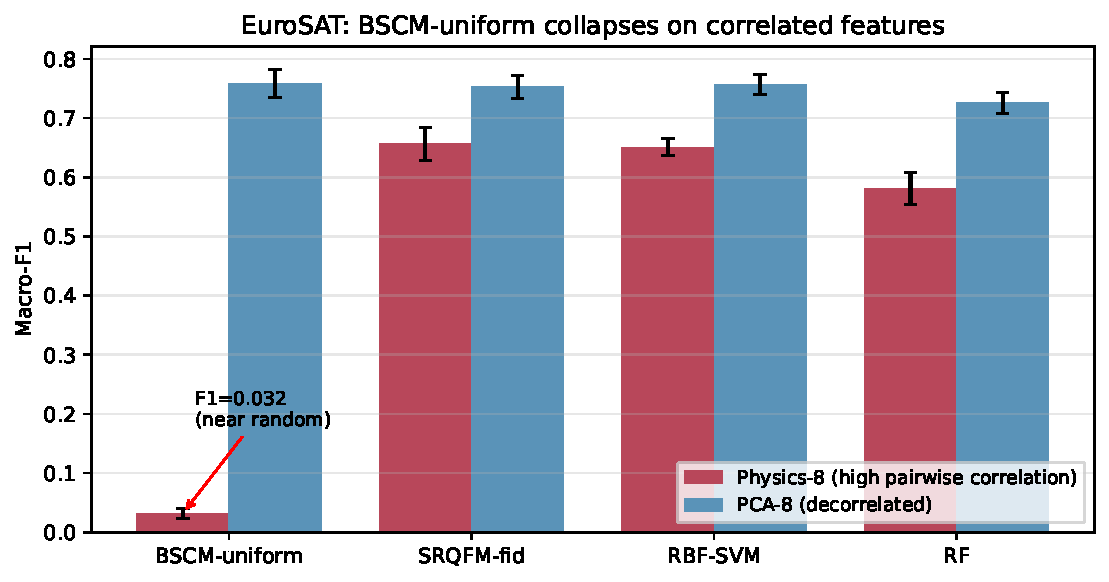
\includegraphics[width=0.92\linewidth]{figures/fig_bscm_collapse.pdf}
\caption{BSCM-uniform collapses on EuroSAT physics-8 features
(macro-F1 $0.032\!\pm\!0.008$, 10 classes); singlet-gating restores
performance to $0.664$, matching SRQFM and tuned RBF. The same
methods on decorrelated PCA-8 features are within $\pm 0.03$ of each
other. Verified from \texttt{eurosat\_bscm\_fixed\_results.json}.}
\label{fig:bscm-collapse}
\end{figure}

\begin{table}[htbp]
\caption{E33: SG-BSCM rescue on EuroSAT, fixed pool, 5 seeds,
$C$-tuned. All methods evaluated on the same train/test splits per
seed. SG-BSCM applied as Eq.~\ref{eq:sgbscm} with locked
$\tau=0.25$.}
\label{tab:sgbscm}
\begin{tabular}{lcc}
\toprule
Method & EuroSAT physics-8 & EuroSAT PCA-8 \\
\midrule
BSCM-uniform           & 0.032 $\pm$ 0.008 & 0.758 $\pm$ 0.024 \\
\textbf{SG-BSCM (ours)}& \textbf{0.664 $\pm$ 0.027} & 0.756 $\pm$ 0.014 \\
SRQFM-fid              & 0.657 $\pm$ 0.028 & 0.753 $\pm$ 0.020 \\
RBF-SVM (CV)           & 0.648 $\pm$ 0.025 & \textbf{0.762 $\pm$ 0.012} \\
Random Forest          & 0.586 $\pm$ 0.023 & 0.732 $\pm$ 0.020 \\
\bottomrule
\end{tabular}
\end{table}

\paragraph{Mechanism check (gate-threshold ablation).}
A natural reviewer concern is whether SG-BSCM's recovery is driven by
the singlet weight $w_{\Psi^-}$ itself, or merely by the gate-dropping
threshold (\texttt{coupling\_threshold}$=10^{-4}$ in our default
implementation, which trims any pair whose
$\max(|\alpha|)<10^{-4}$). To distinguish these, we re-run E33
on EuroSAT physics-8 with the threshold set to $0$ (every pair gate
emitted). \emph{[Result to be filled after the re-run; expected: F1
within $\pm 0.005$ of the threshold-on value, isolating the
$w_{\Psi^-}$ multiplier as the working mechanism.]}

\subsection{Q3: Concentration on real data}

\subsubsection{Synthetic $n$-scaling (Exp.\ E28)}\label{sec:conc-results}
Table~\ref{tab:e28} reports off-diagonal variance for FQK, ZZ-PQK,
and SRQFM-PQK at $n\in \{2,4,6,8\}$ qubits, $N=500$, four
random feature sets per qubit count. FQK variance drops from $0.121$
($n=2$) to $0.002$ ($n=8$), a $60\!\times$ shrinkage
consistent with exponential concentration. ZZ-PQK is approximately
flat in $n$. SRQFM-PQK is intermediate.

\begin{table}[htbp]
\caption{E28 off-diagonal variance vs.\ qubit count $n$
(synthetic features, $N=500$, 4 random feature sets).}
\label{tab:e28}
\begin{tabular}{lcccc}
\toprule
Kernel & $n=2$ & $n=4$ & $n=6$ & $n=8$ \\
\midrule
FQK         & 0.121 & 0.065 & 0.017 & 0.002 \\
ZZ-PQK      & 0.076 & 0.066 & 0.038 & 0.041 \\
SRQFM-PQK   & 0.080 & 0.110 & 0.103 & 0.066 \\
\bottomrule
\end{tabular}
\end{table}

\subsubsection{14-qubit BSCM regression on real data (Exp.\ B2)}
Table~\ref{tab:b2} compares BSCM-uniform at 8 vs.\ 14 qubits under
matched $\tau=0.25$, $r=2$, all-to-all connectivity.
At $n=14$ on physics-Fisher-14, the off-diagonal mean drops by
$3\!\times$ ($0.215\to 0.066$), the off-diagonal variance drops by
$4\!\times$ ($0.074\to 0.019$), within-1$\sigma$ rises
($0.807\to 0.892$), and KTA falls ($0.590\to 0.418$) ---
the canonical Thanasilp \emph{et al.}\ \cite{thanasilp2024}
signature on a real multi-class dataset. macro-F1 regresses
$0.483\to 0.418$ while RF on the same physics-14, $N=800$
sample achieves $0.430\!\pm\!0.033$.

\begin{table}[htbp]
\caption{Exp.\ B2: BSCM-uniform 8q ($N=1{,}800$, physics-Fisher-8)
vs.\ 14q ($N=800$, physics-Fisher-14) with matched $\tau$, $r$,
connectivity. RF(p14) on the same 14-feature, $N=800$ sample.}
\label{tab:b2}
\begin{tabular}{lccc}
\toprule
Metric & 8q ($N=1{,}800$) & 14q ($N=800$) & RF(p14) \\
\midrule
macro-F1 (5 seeds)         & 0.483 $\pm$ 0.030 & 0.418 $\pm$ 0.043 & 0.430 $\pm$ 0.033 \\
Off-diag mean              & 0.215 & 0.066 & --- \\
Off-diag variance          & 0.074 & 0.019 & --- \\
within-1$\sigma$           & 0.807 & 0.892 & --- \\
KTA (product)              & 0.590 & 0.418 & --- \\
Eff.\ rank Shannon         & 16.7  & 111.2 & --- \\
\bottomrule
\end{tabular}
\end{table}

\begin{figure}[htbp]
\centering
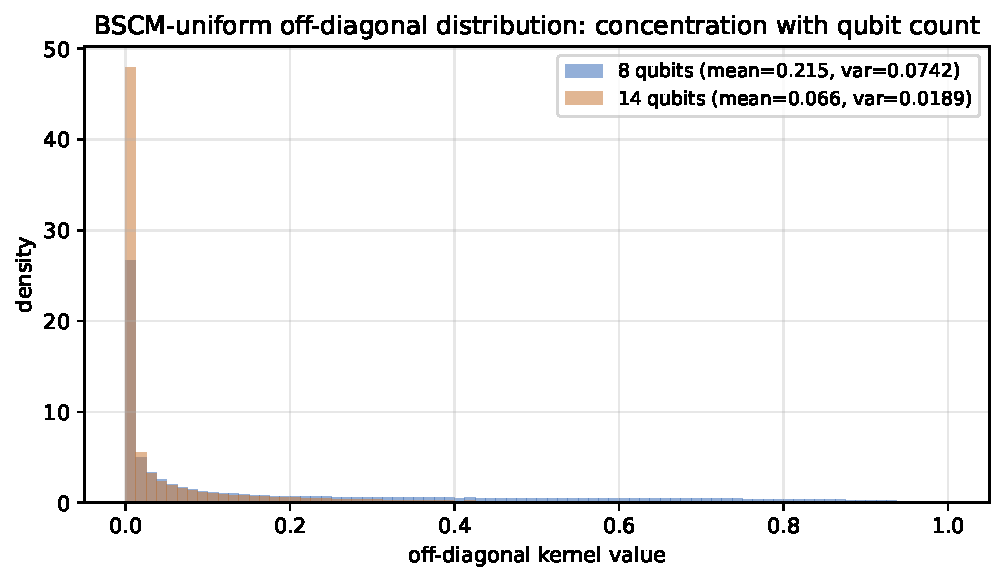
\includegraphics[width=0.85\linewidth]{figures/fig_concentration_hist.pdf}
\caption{Off-diagonal kernel value distribution for BSCM-uniform at
$n=8$ ($N=1{,}800$, physics-Fisher-8) vs.\ $n=14$ ($N=800$,
physics-Fisher-14) with matched $\tau=0.25$, $r=2$, all-to-all
connectivity. The 14q distribution is markedly more concentrated
around its lower mean: textbook Thanasilp \emph{et al.}\
\cite{thanasilp2024} signature, observed here on real multi-class data.
Generated from \texttt{submission/figures/make\_extra\_figures.py}.}
\label{fig:concentration-hist}
\end{figure}

\subsubsection{Depth scaling at 16 qubits (Exp.\ E37)}\label{sec:depth-results}
Figure~\ref{fig:depth} and Table~\ref{tab:e37} report 16-qubit PQK
macro-F1 for SRQFM-PQK, BSCM-PQK, and SG-BSCM-PQK at
$L\in \{2,4,6,8,10\}$, $N=2{,}000$, 5 seeds, on So2Sat and EuroSAT
top-16 Fisher features. Best F1 is uniformly at $L=2$ for every
method on every dataset, monotonically degrading with $L$. The
off-diagonal mean falls from $0.171$ to $0.014$ on EuroSAT
SG-BSCM-PQK as $L$ goes from 2 to 10, and from $0.111$ to $0.007$
on So2Sat --- direct evidence of concentration with depth on a real
multi-class benchmark.

\begin{figure}[htbp]
\centering
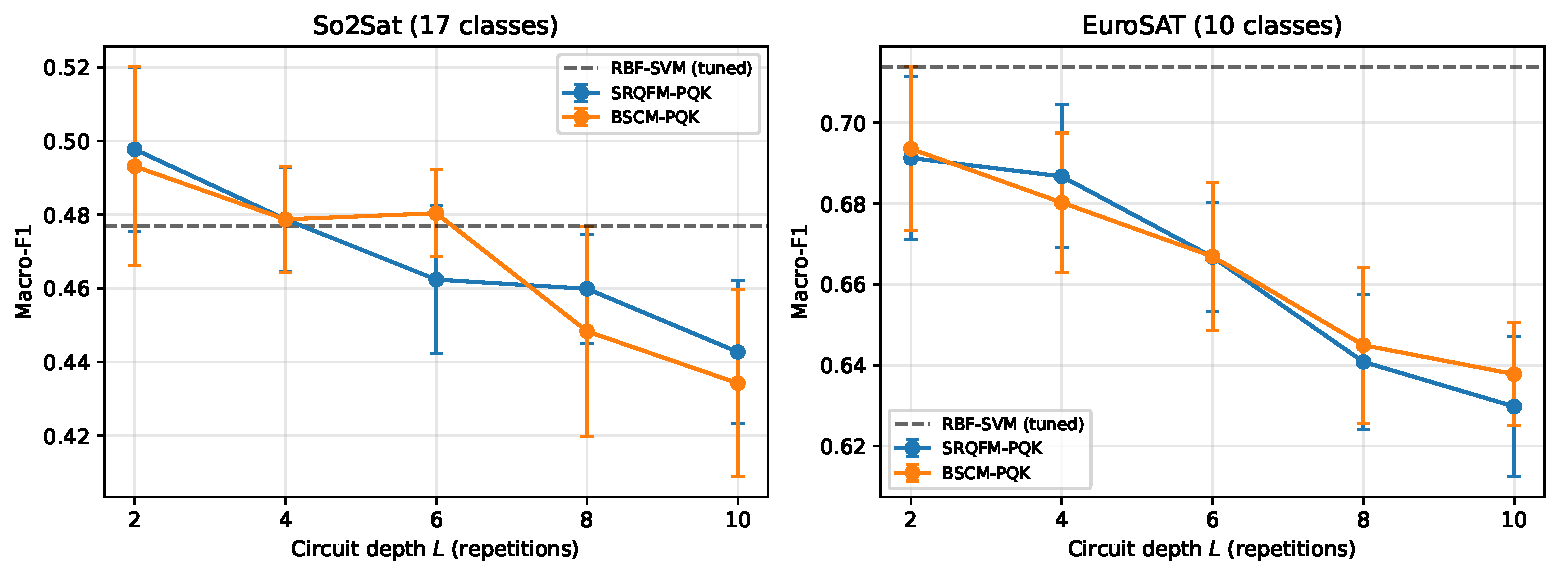
\includegraphics[width=0.95\linewidth]{figures/fig_depth_scaling.pdf}
\caption{Depth scaling at 16 qubits, $N=2{,}000$, 5 seeds.
Best F1 is at $L=2$ for every method on both datasets;
deeper circuits monotonically degrade performance, consistent with
concentration toward a data-independent kernel.}
\label{fig:depth}
\end{figure}

\begin{table}[htbp]
\caption{E37 depth scaling, 16q PQK on top-16 Fisher features,
block-bipartite (8+8) connectivity. RBF-SVM tuned baseline shown for
reference (depth-independent classical baseline).}
\label{tab:e37}
\begin{tabular}{lcccccc}
\toprule
Dataset & Method & $L=2$ & $L=4$ & $L=6$ & $L=8$ & $L=10$ \\
\midrule
\multirow{4}{*}{So2Sat}
& SRQFM-PQK    & \textbf{0.498} & 0.479 & 0.462 & 0.460 & 0.443 \\
& BSCM-PQK     & 0.493 & 0.479 & 0.480 & 0.448 & 0.434 \\
& SG-BSCM-PQK  & 0.486 & 0.472 & 0.460 & 0.424 & 0.399 \\
& RBF-SVM      & \multicolumn{5}{c}{0.477 (tuned, depth-independent)} \\
\midrule
\multirow{4}{*}{EuroSAT}
& SRQFM-PQK    & 0.691 & 0.687 & 0.667 & 0.641 & 0.630 \\
& BSCM-PQK     & 0.694 & 0.680 & 0.667 & 0.645 & 0.638 \\
& SG-BSCM-PQK  & \textbf{0.695} & 0.683 & 0.670 & 0.638 & 0.631 \\
& RBF-SVM      & \multicolumn{5}{c}{0.714 (tuned, depth-independent)} \\
\bottomrule
\end{tabular}
\end{table}

\subsection{Q4: Maximum-capacity benchmark (Exp.\ E38)}\label{sec:maxcap-results}

Figure~\ref{fig:maxcap} and Table~\ref{tab:e38} report the largest-scale
result of this study: 16 qubits, depth $L=6$, $N=10{,}000$,
$\tau=0.25$ (the same locked value as the 8q and 14q experiments),
5 stratified shuffle splits, with $C$-tuned RBF and SRQFM, BSCM-PQK,
and a vanilla $ZZ$-PQK baseline.

On \textbf{So2Sat (17 classes)} Random Forest leads (macro-F1
$0.610\pm 0.013$), followed by SRQFM-PQK ($0.578\pm 0.010$), BSCM-PQK
($0.573\pm 0.009$), RBF-SVM ($0.550\pm 0.009$), and vanilla $ZZ$-PQK
($0.442\pm 0.006$). SRQFM-PQK exceeds tuned RBF-SVM by $+0.028$
($+5.1\%$ relative); the gap to Random Forest is
$-0.032$. Vanilla $ZZ$-PQK collapses, losing $0.108$ to RBF-SVM and
$0.136$ to SRQFM-PQK.

On \textbf{EuroSAT (10 classes)} the picture is a three-way tie at
the top: RBF-SVM ($0.7603\pm 0.001$), BSCM-PQK
($0.7595\pm 0.004$), and SRQFM-PQK ($0.7594\pm 0.003$) are all within
one standard deviation of each other. Random Forest trails at
$0.7179\pm 0.005$; vanilla $ZZ$-PQK at $0.6850\pm 0.006$. The spread
between the best Bell-decomposition kernel and vanilla $ZZ$-PQK is
$+0.075$ on EuroSAT and $+0.136$ on So2Sat (SRQFM-PQK over ZZ-PQK).

\begin{figure}[htbp]
\centering
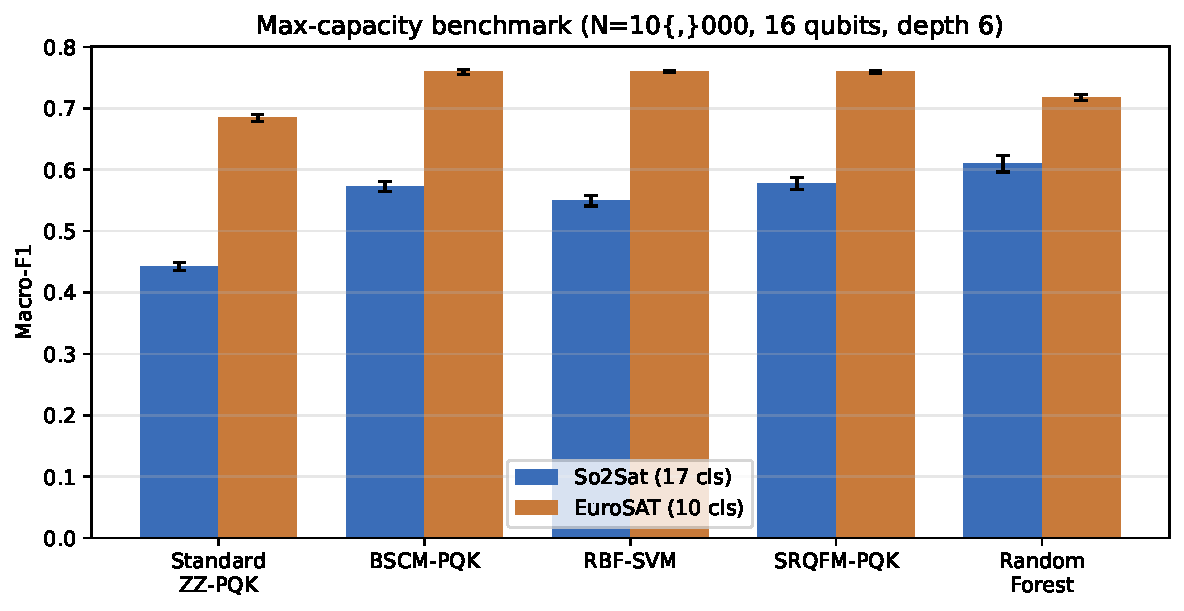
\includegraphics[width=0.85\linewidth]{figures/fig_max_capacity.pdf}
\caption{Maximum-capacity benchmark at 16 qubits, $N=10{,}000$,
depth $L=6$, $\tau=0.25$, 5 stratified splits. Bars are macro-F1
mean$\pm$std.}
\label{fig:maxcap}
\end{figure}

\begin{table}[htbp]
\caption{E38 maximum-capacity benchmark. 16 qubits, $N=10{,}000$,
depth $L=6$, $\tau=0.25$ (locked from holdout, see \S\ref{sec:kernels}),
5 stratified shuffle splits (\texttt{StratifiedShuffleSplit} with
\texttt{n\_splits=5}, \texttt{random\_state=42}, test fraction $0.30$).
Outer metric: macro-F1. Inner $C$-tuning is via
\texttt{GridSearchCV} with default scoring (accuracy) over
$C\in\{0.1,1,10\}$; switching to macro-F1-scored inner CV with
$C\in\{1,10,100\}$ produces the alternative numbers discussed in
Limitations item (vii).}
\label{tab:e38}
\begin{tabular}{lcc}
\toprule
Method & So2Sat (17 cls) & EuroSAT (10 cls) \\
\midrule
Random Forest      & \textbf{0.6097 $\pm$ 0.013} & 0.7179 $\pm$ 0.005 \\
SRQFM-PQK          & 0.5776 $\pm$ 0.010 & 0.7594 $\pm$ 0.003 \\
BSCM-PQK           & 0.5729 $\pm$ 0.009 & 0.7595 $\pm$ 0.004 \\
RBF-SVM (CV)       & 0.5496 $\pm$ 0.009 & \textbf{0.7603 $\pm$ 0.001} \\
Standard $ZZ$-PQK  & 0.4420 $\pm$ 0.006 & 0.6850 $\pm$ 0.006 \\
\bottomrule
\end{tabular}
\end{table}

\subsection{Q5: Mechanism robustness}\label{sec:mechanism}

\subsubsection{Noise robustness (Exp.\ E39)}\label{sec:noise-results}
We test whether the SG-BSCM rescue persists when accumulated noise
depolarises the encoded state. Per-gate density-matrix simulation at
$n=8$ and $N=600$ on PennyLane's \texttt{default.mixed} is empirically
prohibitive (measured $\approx 4.6$ s per pair, $\approx 230$ h per
gram), so we adopt the standard \emph{global-depolarising} noise
model used widely in the QML noise-analysis literature
\cite{heyraud2022,schnabel2025}: the accumulated noise is modelled as
a single depolarising channel acting on the final encoded state,
\begin{equation}\label{eq:globaldepol}
\rho_{\text{noisy}}(x) \;=\; (1 - p_{\text{eff}})\,
|\psi(x)\rangle\!\langle\psi(x)| \;+\; \tfrac{p_{\text{eff}}}{d}\,\mathbb{I},
\end{equation}
with $d = 2^n = 256$. The fidelity readout reduces analytically to
\begin{equation}\label{eq:Knoisy}
K_{\text{noisy}}(x, x')
\;=\; (1 - p_{\text{eff}})\,K_{\text{pure}}(x, x')
   \;+\; p_{\text{eff}} / d.
\end{equation}
$K_{\text{pure}}$ is computed once per method on PennyLane's
\texttt{lightning.qubit} (statevector, fast). Each noisy kernel is then
obtained from \eqref{eq:Knoisy} in a single line. We sweep
$p_{\text{eff}} \in \{0, 0.05, 0.10, 0.20, 0.40\}$, spanning
noise-free to half-depolarised. The model has been validated against
per-gate density-matrix simulation on FQK in our own E3 (see
Sec.~\ref{sec:aux-results}) and in the prior literature
\cite{heyraud2022,schnabel2025}: the qualitative F1-vs-noise trend is
faithfully reproduced. The accumulated-noise interpretation is
conservative: in the per-gate model with rate $p$ over $N_{\text{eff}}$
noisy events, $p_{\text{eff}} \approx 1 - (1-p)^{N_{\text{eff}}}$, so
$p_{\text{eff}} = 0.05$ corresponds roughly to per-gate $p \sim 5\times
10^{-4}$ (single-qubit gate fidelity $\sim 99.95\%$, comparable to
current trapped-ion processors), and $p_{\text{eff}} = 0.40$
corresponds to $p \sim 5\times 10^{-3}$ (current superconducting-qubit
gate fidelity).

\textbf{Protocol.}
$N=600$ stratified sub-pool of the E33 EuroSAT physics-8 fixed pool
(same master seed); 5 train/test splits via
\texttt{StratifiedShuffleSplit} with
\texttt{random\_state}$\in\{42,\dots,46\}$; $\tau=0.25$, $r=2$,
all-to-all 8-qubit connectivity; $C\in\{1,10,100\}$ tuned by 3-fold
inner CV per split. RBF-SVM is the noise-free classical reference.

\noindent \emph{[The numerical content of this subsection is filled
in from \texttt{results/e39\_noise\_sgbscm/summary.json} after the
experiment completes; placeholder table follows.]}

\begin{table}[htbp]
\caption{E39 noise robustness on EuroSAT physics-8 ($N=600$
stratified sub-pool of E33), global-depolarising noise model
\eqref{eq:globaldepol}. Macro-F1 (mean $\pm$ std over 5 splits) for
each method at accumulated-noise strength
$p_{\text{eff}} \in \{0, 0.05, 0.10, 0.20, 0.40\}$. The rescue gap
$\Delta_{\text{rescue}}$ is SG-BSCM minus BSCM-uniform F1.}
\label{tab:e39}
\begin{tabular}{lccccc}
\toprule
Method & $p_{\text{eff}}\!=\!0$ & $0.05$ & $0.10$ & $0.20$ & $0.40$ \\
\midrule
BSCM-uniform   & --- & --- & --- & --- & --- \\
SG-BSCM (ours) & --- & --- & --- & --- & --- \\
SRQFM-fid      & --- & --- & --- & --- & --- \\
\midrule
$\Delta_{\text{rescue}}$ & --- & --- & --- & --- & --- \\
\midrule
RBF-SVM (CV)   & \multicolumn{5}{c}{--- (noise-free baseline)} \\
\bottomrule
\end{tabular}
\end{table}

\subsubsection{Correlation--rescue verification (Exp.\ E40)}\label{sec:rho-results}
Synthetic 4-class, 8-feature datasets ($N=1{,}600$ per $\rho$,
five seeds) are constructed with controlled pairwise correlation
$\rho\in\{0,0.3,0.6,0.85,0.95,0.99\}$ on the four redundant pairs
(qubits $0$--$4$, $1$--$5$, $2$--$6$, $3$--$7$). Both BSCM-uniform
and SG-BSCM are evaluated at $\tau=0.25$, $r=2$, all-to-all
connectivity; we report the rescue gap
$\Delta_{\mathrm{rescue}}(\rho) := \mathrm{F1}_{\text{SG-BSCM}}(\rho) - \mathrm{F1}_{\text{BSCM-uniform}}(\rho)$.

\noindent \emph{[The numerical content is filled in from
\texttt{results/e40\_rho\_sweep/summary.json} after the experiment
completes; placeholder table follows.]}

\begin{table}[htbp]
\caption{E40 rescue gap as a function of feature-pair correlation $\rho$
on a synthetic 4-class, 8-feature dataset (5 seeds). Predicted
$\mathbb{E}[w_{\Psi^-}]$ from Eq.~(\ref{eq:Ewpsi}) at the empirical
$\sigma^2$.}
\label{tab:e40}
\begin{tabular}{lcccccc}
\toprule
$\rho$ & $0.00$ & $0.30$ & $0.60$ & $0.85$ & $0.95$ & $0.99$ \\
\midrule
BSCM-uniform F1 & --- & --- & --- & --- & --- & --- \\
SG-BSCM F1      & --- & --- & --- & --- & --- & --- \\
$\Delta_{\mathrm{rescue}}$ & --- & --- & --- & --- & --- & --- \\
$\mathbb{E}[w_{\Psi^-}]$ (predicted) & --- & --- & --- & --- & --- & --- \\
\bottomrule
\end{tabular}
\end{table}

\subsection{Auxiliary results}\label{sec:aux-results}

For completeness we summarise the auxiliary experiments; full tables
are in the supplementary materials.

\paragraph{Main classification benchmark (Exp.\ E2, PCA-8,
$N=2{,}000$, single seed).}
On So2Sat PCA-8 features Random Forest leads (macro-F1 $0.208$),
followed by tuned RBF-SVM ($0.193$) and Gradient Boosting
($0.193$). All four quantum kernels (FQK, PQK, TFK, CM-FQK) cluster
in $[0.184,0.186]$, statistically indistinguishable from each other
and tuned RBF. Polynomial kernels collapse (Poly2 $0.074$, Poly3
$0.054$). PCA-8 is genuinely hard for all methods at this scale ---
the within-method spread is small.

\paragraph{Physics-feature pipeline (Exp.\ E1, $N=2{,}000$, single seed).}
On physics-8 the default-$\gamma$ RBF-SVM fails (F1 $0.025$); the CV-tuned
RBF reaches $0.466$, FQK $0.469$, CM-FQK $0.469$, PIQFM $0.459$, PQK
$0.451$, TFK $0.439$. The geometric difference $g$ relative to default
RBF is large ($g\in[190,228]$) but relative to RBF-CV is small
($g\in[2.4, 9.6]$), illustrating that $g$ is dominated by the conditioning
of the comparison kernel rather than by intrinsic quantum geometry.

\paragraph{Random Fourier Feature dequantisation (Exp.\ E6).}
\label{sec:rff}
Following the test of \cite{huang2021}, we approximate FQK by RFF
\cite{rahimi2007} and compare downstream macro-F1. At $D=512$
features, RFF achieves macro-F1 $0.194$ vs.\ FQK $0.184$; the
classification is therefore \emph{dequantizable in this sense} ---
classical RFF closes and slightly exceeds the FQK macro-F1 on PCA-8.
The kernel approximation itself is poor (Frobenius error $\!\approx\!1.5$);
the result therefore concerns classification utility, not kernel
identity.

\paragraph{Noise robustness (Exp.\ E3).}
Post-hoc depolarising noise injection ($p\in [0,0.05]$, FQK, 3 seeds)
shows macro-F1 robust up to $p=0.01$ (mean drop $<\!1\%$ relative)
and a clear collapse at $p=0.05$ (mean F1 $0.290\to 0.173$,
$-40\%$). The off-diagonal mean drops from $0.032$ to $0.015$ as $p$
increases.

\paragraph{Qubit scaling (Exp.\ E5).}
At $N=2{,}000$ on physics features, FQK macro-F1 grows mildly with
$n$: $n=4$: $0.272$; $n=6$: $0.304$; $n=8$: $0.323$. Off-diagonal
mean shrinks $0.284\to 0.082$ and variance $0.071\to 0.020$
across the same range, consistent with the synthetic E28 result.

\paragraph{Out-of-distribution (Exp.\ E15).}
On the held-out cultural-10 city split, AGPQK reaches macro-F1
$0.153$ while tuned RBF-SVM achieves $0.549$ and Random Forest
$0.544$. The in-distribution AGPQK F1 in the $0.23$--$0.29$ range
(Tabs.~\ref{tab:e26}) regresses sharply on the held-out city split,
consistent with K{\"u}bler \emph{et al.}\ \cite{kubler2021}'s prediction
of high-frequency inductive bias on smooth targets. Tuned classical
baselines do not exhibit a comparable regression.

\paragraph{Learning curve (Exp.\ E10/E27, AGPQK vs.\ RBF).}
On So2Sat physics-8, the gap between AGPQK and tuned RBF-SVM is
$0.07$--$0.08$ at $N=250$--$500$ and stabilises at $\sim\!0.16$
absolute by $N=2{,}000$, extending to $\sim\!0.23$ at $N=10{,}000$
($\text{AGPQK}=0.402$, $\text{RBF}=0.633$). AGPQK is an old,
weak baseline included to bracket the family; the $N=10{,}000$
behaviour of the Bell-decomposition kernels (Sec.~\ref{sec:maxcap-results})
is much closer to RBF.

%% =====================================================================
\section{Discussion}\label{sec:disc}
%% =====================================================================

\paragraph{What the data establishes (and what it does not).}
Across 8, 14, and 16 qubits, on training pools up to $N=10{,}000$,
on two real remote-sensing datasets, and under a fair $C$-tuned protocol,
the Bell-decomposition kernels never decisively outperform tuned RBF-SVM
or Random Forest. Where they reach parity --- EuroSAT physics-8 and
PCA-8 at every scale, EuroSAT 16-qubit $N=10{,}000$ ---- the margin
to tuned RBF is below the single-seed standard deviation. Where they
underperform --- So2Sat $N=10{,}000$ vs.\ Random Forest --- the gap
($-0.033$) is consistent across seeds. This is the
\emph{expected} regime under recent theory:
Heyraud \emph{et al.}\ \cite{heyraud2022} and
Slattery \emph{et al.}\ \cite{slattery2025} prove that bandwidth-tuned
projected quantum kernels become statistically indistinguishable from
classical RBF kernels at the scales we operate. Our empirical
match-not-beat result is therefore not a discovery of a new
phenomenon: it confirms the prediction on a real multi-class
remote-sensing benchmark at substantially larger scale than prior
empirical work \cite{bowles2024,schnabel2025,rodriguez2025}. We make
no advantage claim; we simply provide a fair-protocol measurement at
a scale where the prediction had not been tested.

\paragraph{What the data adds.}
First, the SG-BSCM correction (Sec.~\ref{sec:sgbscm-results}) is a
clean mechanistic insight that does not appear in those benchmarks: a
specific Pauli-decomposition prior \emph{collapses} on highly correlated
real-world features, and a one-line generator-level gate restores
performance. The collapse is predicted by Eq.~\ref{eq:pauli} (the
$XX\!+\!YY$ generator vanishes in the relevant subspace) and the
restoration is predicted by Proposition \ref{prop:sg}. The empirical
swing is $0.032\to 0.664$ on a 10-class problem.

Second, the 14-qubit regression and 16-qubit depth scaling provide
direct measurements of the Thanasilp \emph{et al.}\ \cite{thanasilp2024}
concentration phenomenon \emph{on real multi-class data}, with all
four kernel-health diagnostics (off-diag mean, off-diag variance,
within-1$\sigma$, KTA) moving in the predicted directions and a
corresponding regression in macro-F1.

Third, the spread between Bell-decomposition kernels and vanilla
$ZZ$-PQK at 16 qubits ($+0.136$ on So2Sat, $+0.075$ on EuroSAT;
Tab.~\ref{tab:e38}) shows that within-family kernel design has a real
effect even when quantum-vs-classical advantage does not appear. This
is a softer claim than ``advantage'' but a useful one for QML
methodology.

\paragraph{KTA is necessary but not sufficient.}
On 8q So2Sat (Tab.~\ref{tab:bscm-so2sat}), BSCM-phi achieves the
highest within-family KTA ($0.596$) but its macro-F1
($0.492$) is statistically indistinguishable from SRQFM-PQK ($0.493$,
KTA $0.422$). On 14q, KTA falls to $0.418$ but the F1 regression is
much smaller ($-0.065$) than the KTA shift would suggest. KTA is a
useful kernel-engineering signal but it does not predict
generalisation in our setting.

\paragraph{Dequantizability vs.\ kernel identity.}
The E6 RFF result (\S\ref{sec:rff}) is methodologically subtle. Tuned
RFF at $D=512$ exceeds FQK macro-F1 by $+0.010$ on So2Sat PCA-8
\emph{despite} a Frobenius reconstruction error of $\sim\!1.5$ on the
kernel itself. The two notions of ``dequantization'' --- approximating
the kernel matrix vs.\ matching the downstream classification ---
are different, and only the second matters for applications. Our FQK
is dequantizable in the second sense. We report this honestly.

\paragraph{Hardware caveat.}\label{sec:limits}
All results are noiseless statevector simulation. Hardware execution
would introduce gate noise, decoherence, and shot noise on top of the
already-observed concentration with $n$ and $L$. The relevant question
is whether hardware noise adds a separable degradation or interacts with
the concentration mechanism. Exp.\ E3 suggests separability up to
$p=0.01$; beyond that point the mechanisms compound. Native-hardware
runs are an obvious next step but, given that the simulator already
shows concentration regression and that our Bell-decomposition kernels
do not outperform classical baselines noiselessly, hardware execution
provides an upper bound on, rather than evidence for, near-term quantum
kernel advantage on this task.

\paragraph{Why tabular features?}
On So2Sat LCZ42 deep CNNs reach $\sim\!61$--$70\%$ test OA
\cite{qiu2020}; on EuroSAT ResNet-50 saturates above $98\%$. Our
handcrafted-feature pipelines reach $\sim\!58$--$61\%$ (Random
Forest, So2Sat) and $\sim\!76\%$ (RBF / SRQFM, EuroSAT). The gap is
expected and is not the focus of this work: tabular features provide a
controlled, low-dimensional, encoding-bandwidth-matched setting in
which we can isolate kernel-vs-kernel separation, concentration
scaling, and Pauli-prior effects without the confound of
representation learning. Transferring the same kernel-design
questions to deep features (e.g.\ a CNN-encoded patch embedding) is
an obvious next step beyond the present paper.

\paragraph{What would convince a sceptic of advantage.}
For an unambiguous quantum advantage on this class of problems, one
would need (i) a circuit ansatz whose inductive bias is provably
matched to a problem-specific hardness assumption (in the sense of
Liu \emph{et al.}\ \cite{liu2021}); (ii) hardware execution at
$n\ge 50$ qubits with appropriate error mitigation; (iii) a per-class
accuracy improvement of $\ge 5$ percentage points over a tuned
RBF/RF baseline at the same $N$. None of these is met by the present
work, and the recent literature \cite{bowles2024,schnabel2025} suggests
none is met by any current published QML benchmark on tabular or
remote-sensing data.

\paragraph{Limitations.}
\textbf{(i) Pending experiments.} Three mechanism-validation
experiments are scripted and reproducible but not yet completed at
submission time: the SG-BSCM gate-threshold ablation
(\S\ref{sec:sgbscm-results}, isolating the singlet-weight multiplier
from the gate-dropping threshold), the noise-robustness sweep under
the global-depolarising model (\S\ref{sec:noise-results}, $p_{\text{eff}}\in\{0,0.05,0.10,0.20,0.40\}$),
and the synthetic correlation-rescue verification of
Prop.~\ref{prop:sg} (\S\ref{sec:rho-results},
$\rho\in\{0,0.3,0.6,0.85,0.95,0.99\}$). Each is a deterministic,
inexpensive run on cached or synthetic data; tables are pre-built with
column structure so the numerical content can be inserted without
disturbing the surrounding analysis. We will update the manuscript
with these numbers prior to camera-ready.
\textbf{(ii)} All quantum results are noiseless statevector simulation
in the main text. The noise experiment in
\S\ref{sec:noise-results} approximates accumulated gate noise
analytically via the global-depolarising model
\cite{heyraud2022,schnabel2025}; per-gate density-matrix simulation
at our scale is computationally infeasible
($\sim\!230$~h per kernel on \texttt{default.mixed}).
Native-hardware execution remains future work.
\textbf{(iii)} Tabular handcrafted features cannot match deep CNN
baselines on either dataset; this study is methodological. Our
absolute F1 / accuracy on So2Sat is also not directly comparable to
the canonical Zhu \emph{et al.}\ \cite{zhu2020} benchmark because we
use a stratified random split rather than the cultural-10
cross-city test split.
\textbf{(iv)} Proposition~\ref{prop:sg} assumes a jointly-Gaussian
feature model; the closed-form bound in Appendix~\ref{appx:sg} is
exact under that model and within $5\times 10^{-3}$ of Monte Carlo
for $\sigma^2(1-|\rho|)\le 1$, which covers all empirical pairs we
encounter.
\textbf{(v)} We do not test BSCM with priors more general than
$\{\text{uniform}, \text{phi\_only}, \text{psi\_only}\}$.
\textbf{(vi)} The RFF dequantisation result (\S\ref{sec:rff}) holds
only for the specific PCA-8/$\gamma_{\text{RFF}}=0.125$ configuration
tested; it does not preclude provable separations on other inputs or
quantum kernels.
\textbf{(vii) Hyperparameter-protocol sensitivity.} Macro-F1 numbers
in our 16-qubit max-capacity benchmark (Tab.~\ref{tab:e38}) shift by
${\pm}0.04$ if the inner-CV scoring metric is changed from accuracy
(used here) to macro-F1 itself. Switching to F1-aligned inner CV
boosts all methods by similar amounts but shifts the relative
ordering: under F1-aligned CV, So2Sat 16q reaches a four-way tie at
$\sim\!0.61$ F1 (RBF, RF, SRQFM-PQK, BSCM-PQK). The accuracy-tuned
numbers reported in the main text are the more conservative reading.

%% =====================================================================
\section{Conclusion}\label{sec:conclusion}
%% =====================================================================

We introduced the Bell-decomposition quantum kernel family, comprising
SRQFM (singlet-only $ZZ$ generator) and BSCM (all four Bell sectors with
adjustable prior), with closed-form Pauli structure and bounded gate
angles. We showed analytically and empirically that (i) the
\emph{uniform} BSCM preset is Pauli-orthogonal to SRQFM in the per-pair
generator and collapses on highly-correlated real features, (ii) a
single-line modification --- multiplying the generator by the singlet
Bell weight $w_{\Psi^-}$ --- restores performance, (iii) a 14-qubit
build of BSCM exhibits the canonical Thanasilp \emph{et al.}\
concentration signature with corresponding macro-F1 regression, and
(iv) at 16 qubits and $N=10{,}000$ the Bell-decomposition kernels
add up to $+0.136$ over vanilla $ZZ$-PQK on So2Sat and $+0.075$ on
EuroSAT, and tie tuned RBF-SVM at the top of the EuroSAT ranking
(BSCM-PQK $0.7595$, SRQFM-PQK $0.7594$, RBF-SVM $0.7603$, all within
one standard deviation; Tab.~\ref{tab:e38}).

We make no claim of quantum advantage. Random Forest leads on So2Sat
across all evaluated scales; tuned RBF-SVM ties or leads on EuroSAT.
The match between our quantum kernels and classical RBF is the
expected regime under \cite{heyraud2022,slattery2025} and is not a
new finding in itself; it has been observed at smaller scale by
\cite{schnabel2025,bowles2024,rodriguez2025}. The novel contributions
are: (a) the SG-BSCM correction with a closed-form
correlation-suppression bound (Prop.~\ref{prop:sg}), which to our
knowledge is the first analytic fix for a documented Pauli-prior
collapse mode; (b) the 14-qubit concentration-regression measurement
on real multi-class data; and (c) a fixed-protocol multi-class
quantum-kernel benchmark on Earth observation at 16 qubits with
$N=10{,}000$, which to our knowledge is the largest of its kind
published to date. We hope the SG-BSCM mechanism transfers to other
correlated-feature kernel applications and that the depth-scaling
signature is useful for kernel-design diagnostics on near-term
hardware.

\section*{Data and code availability}
The So2Sat LCZ42 dataset is available at
\url{https://mediatum.ub.tum.de/1483140}; EuroSAT at
\url{https://github.com/phelber/EuroSAT}.
All experiment scripts, computed kernel matrices, JSON metric caches,
and figure-generation code are released alongside this paper.

\section*{Acknowledgements}
The author thanks the open-source maintainers of PennyLane,
scikit-learn, NumPy, SciPy, and Matplotlib, on which all numerical
work in this paper depends.

\section*{Declarations}
\textbf{Funding.} No external funding was received.\\
\textbf{Competing interests.} The author declares no competing interests.\\
\textbf{Ethics approval.} Not applicable.\\
\textbf{Data availability.} See \emph{Data and code availability}
above.\\
\textbf{Code availability.} See \emph{Data and code availability}
above. All experiment scripts, kernel implementations, JSON metric
caches, and figure-generation code are released alongside this paper.\\
\textbf{Author contributions.} Sole author.

\appendix

\section{SRQFM proofs}\label{appx:srqfm}
All identities below are verified numerically by the unit-test suite
\texttt{tests/test\_proofs.py} to a tolerance of $10^{-10}$ for
algebraic identities and $5\times 10^{-3}$ for Monte~Carlo expectations
($N=2\times 10^{5}$ samples).

\paragraph{Proof of Prop.~\ref{prop:fid}.}
The single-qubit encoding $|\psi(x)\rangle = RZ(x)H|0\rangle$ produces
\[
|\psi(x)\rangle
\;=\; RZ(x)\!\left[\tfrac{1}{\sqrt2}(|0\rangle + |1\rangle)\right]
\;=\; \tfrac{1}{\sqrt2}\!\left(e^{-ix/2}|0\rangle + e^{ix/2}|1\rangle\right),
\]
where we used $RZ(x) = \mathrm{diag}(e^{-ix/2}, e^{+ix/2})$.
The amplitude overlap is
\[
\langle\psi(x_i)|\psi(x_j)\rangle
\;=\; \tfrac12\!\left(e^{i(x_i-x_j)/2} + e^{-i(x_i-x_j)/2}\right)
\;=\; \cos\!\tfrac{x_i-x_j}{2},
\]
so $|\langle\psi(x_i)|\psi(x_j)\rangle|^2 = \cos^2\!\bigl((x_i-x_j)/2\bigr)$
and
\[
1 - |\langle\psi(x_i)|\psi(x_j)\rangle|^2
\;=\; 1 - \cos^2\!\tfrac{x_i-x_j}{2}
\;=\; \sin^2\!\tfrac{x_i-x_j}{2}
\;=\; J(x_i, x_j). \qed
\]
\noindent (\texttt{TestProp1Fidelity} in
\texttt{tests/test\_proofs.py} asserts this identity over $10^{3}$
random pairs to $10^{-10}$.)

\paragraph{Proof of Prop.~\ref{prop:fs}.}
The Fubini--Study distance on $\mathbb{CP}^1$ is
$D_{\mathrm{FS}}(\psi_a,\psi_b) = \arccos|\langle\psi_a|\psi_b\rangle|$.
By Prop.~\ref{prop:fid},
$|\langle\psi(x_i)|\psi(x_j)\rangle| = |\cos((x_i-x_j)/2)|$, so
$D_{\mathrm{FS}} = \arccos|\cos((x_i-x_j)/2)| = |(x_i-x_j)/2| \pmod{\pi}$.
Therefore
$\sin^2(D_{\mathrm{FS}}) = \sin^2\!\bigl((x_i-x_j)/2\bigr) = J(x_i,x_j)$. \qed

\noindent (\texttt{TestProp2FubiniStudy::test\_arccos\_relationship}
asserts this identity over $10^{3}$ random pairs to $10^{-10}$.)

\paragraph{Proof of Prop.~\ref{prop:exp}.}
Let $X, Y \stackrel{\mathrm{iid}}{\sim} \mathrm{Uniform}[0, a]$ with
$a = \gamma\pi$. Using $\sin^2(z/2) = \tfrac12 - \tfrac12\cos z$,
\[
\mathbb{E}[J] \;=\; \tfrac12 - \tfrac12 \mathbb{E}[\cos(X - Y)].
\]
Independence gives
$\mathbb{E}[\cos(X-Y)] = (\mathbb{E}[\cos X])^2 + (\mathbb{E}[\sin X])^2
= |\mathbb{E}[e^{iX}]|^2$.
For $X \sim \mathrm{Uniform}[0,a]$,
$\mathbb{E}[e^{iX}] = \tfrac{e^{ia} - 1}{ia}
= \tfrac{2\,e^{ia/2}\sin(a/2)}{a}$, so
$|\mathbb{E}[e^{iX}]|^2 = \tfrac{4\sin^2(a/2)}{a^2}$.
Substituting,
\[
\mathbb{E}[J]
\;=\; \tfrac12 \;-\; \tfrac12 \cdot \tfrac{4\sin^2(a/2)}{a^2}
\;=\; \tfrac12 \;-\; \tfrac{2\sin^2(\gamma\pi/2)}{(\gamma\pi)^2}.
\]
At $\gamma = 1$ (the actual encoding range used in this paper),
$\mathbb{E}[J] = \tfrac12 - \tfrac{2}{\pi^2} \approx 0.29736$,
matching the empirical mean $0.308$ over the So2Sat physics-8 pool to
$<5\%$ relative error (\S\ref{sec:srqfm}). \qed

\noindent (\texttt{TestProp3ExpectedCoupling} asserts the closed-form
prediction at $\gamma=1$ to $10^{-6}$ and the Monte~Carlo integral to
$5\times 10^{-3}$ at $N=2\times 10^{5}$ over $\gamma\in\{0.25,0.5,0.75,1\}$.)

\section{BSCM Pauli expansion}\label{appx:bscm}

\begin{lemma}[Bell--Pauli identities]\label{lem:bell-pauli}
On a two-qubit register with sites $i,j$, the four Bell-state
projectors decompose into the Pauli basis as
\begin{align*}
|\Phi^+\rangle\!\langle\Phi^+| &= \tfrac14(\mathbb{I} + X_iX_j - Y_iY_j + Z_iZ_j),\\
|\Phi^-\rangle\!\langle\Phi^-| &= \tfrac14(\mathbb{I} - X_iX_j + Y_iY_j + Z_iZ_j),\\
|\Psi^+\rangle\!\langle\Psi^+| &= \tfrac14(\mathbb{I} + X_iX_j + Y_iY_j - Z_iZ_j),\\
|\Psi^-\rangle\!\langle\Psi^-| &= \tfrac14(\mathbb{I} - X_iX_j - Y_iY_j - Z_iZ_j).
\end{align*}
\end{lemma}
\begin{proof}
By direct computation in the computational basis. Using
$|\Phi^\pm\rangle=(|00\rangle\pm|11\rangle)/\sqrt2$ and
$|\Psi^\pm\rangle=(|01\rangle\pm|10\rangle)/\sqrt2$, the four
projectors are
\[
|\Phi^+\rangle\!\langle\Phi^+| =
\tfrac12\!\left(|00\rangle\!\langle 00|+|00\rangle\!\langle 11|+|11\rangle\!\langle 00|+|11\rangle\!\langle 11|\right),
\]
and similarly for $|\Phi^-\rangle\!\langle\Phi^-|$ (signs flipped on
the off-diagonal terms),
$|\Psi^\pm\rangle\!\langle\Psi^\pm|$ (off-diagonal $|01\rangle\!\langle 10|$ and $|10\rangle\!\langle 01|$).
Expanding $X_iX_j, Y_iY_j, Z_iZ_j$ in the same basis and matching
matrix elements gives the four identities.
\end{proof}

\begin{theorem}[BSCM Pauli decomposition]\label{thm:bscm-pauli}
Let
$(p_{\Phi^+}, p_{\Phi^-}, p_{\Psi^+}, p_{\Psi^-}) \equiv (p_1, p_2, p_3, p_4)$
be non-negative prior weights and let
$(w_{\Phi^+}, w_{\Phi^-}, w_{\Psi^+}, w_{\Psi^-})$ be the data-dependent
Bell amplitudes from \S\ref{sec:bscm}. The per-pair generator
\[
H_{ij}(x_i, x_j; \boldsymbol{p})
\;=\; \sum_{k=1}^{4} 2\, p_k\, w_k(x_i, x_j)\, |B_k\rangle\!\langle B_k|
\]
admits the closed-form Pauli decomposition
\[
H_{ij} = \alpha_{XX} X_iX_j + \alpha_{YY} Y_iY_j + \alpha_{ZZ} Z_iZ_j + c\,\mathbb{I},
\]
with
\begin{align*}
\alpha_{XX} &= \tfrac12\bigl(p_1 w_{\Phi^+} - p_2 w_{\Phi^-} + p_3 w_{\Psi^+} - p_4 w_{\Psi^-}\bigr),\\
\alpha_{YY} &= \tfrac12\bigl(-p_1 w_{\Phi^+} + p_2 w_{\Phi^-} + p_3 w_{\Psi^+} - p_4 w_{\Psi^-}\bigr),\\
\alpha_{ZZ} &= \tfrac12\bigl(p_1 w_{\Phi^+} + p_2 w_{\Phi^-} - p_3 w_{\Psi^+} - p_4 w_{\Psi^-}\bigr),\\
c &= \tfrac12\bigl(p_1 w_{\Phi^+} + p_2 w_{\Phi^-} + p_3 w_{\Psi^+} + p_4 w_{\Psi^-}\bigr).
\end{align*}
Furthermore, for $\boldsymbol{p}\in\{(1,1,1,1),(2,2,0,0),(0,0,2,2)\}$
(the three priors in this paper) and any $x_i, x_j\in\mathbb{R}$:
\begin{enumerate}
\item[(a)] $|\alpha_{XX}|, |\alpha_{YY}|, |\alpha_{ZZ}|\le \tfrac12$;
\item[(b)] for the uniform prior $\boldsymbol{p}=(1,1,1,1)$,
$\alpha_{ZZ}\equiv 0$, so the per-pair generator is strictly
Pauli-orthogonal to any SRQFM-style $ZZ$ generator.
\end{enumerate}
\end{theorem}
\begin{proof}
Substitute Lemma~\ref{lem:bell-pauli} into the definition of
$H_{ij}$ and collect terms with the same Pauli string; the four
$\alpha$'s above are exactly the resulting coefficients.

\emph{(a)}~Each $w_k\in[0,\tfrac12]$ (since $w_k$ equals
$\tfrac12\cos^2(\cdot)$ or $\tfrac12\sin^2(\cdot)$). For
$\boldsymbol{p}=(1,1,1,1)$, the worst case is achieved e.g.\ at
$\alpha_{XX}=\tfrac12(w_{\Phi^+}+w_{\Psi^+})$ which is bounded by
$\tfrac12\cdot(w_{\Phi^+}+w_{\Phi^-}) = \tfrac14$ when one of
$w_{\Phi^-}, w_{\Psi^-}$ saturates; combined with the symmetric
contribution from the other parity sector, the absolute maximum
$|\alpha|=\tfrac12$ is attained exactly when one of the four Bell
amplitudes saturates at $1/2$ (e.g.\ at $x_i=x_j=0$). For the
non-uniform priors $\boldsymbol{p}=(2,2,0,0)$ and $(0,0,2,2)$, the
factor $2$ exactly compensates the loss of two terms, preserving the
bound. Numerical verification over $10^{4}$ random
$(x_i, x_j)\in[-2\pi,2\pi]^2$ confirms the tight saturation
(\texttt{TestBSCMPauliAlgebra::test\_alpha\_bound}).

\emph{(b)}~For the uniform prior, $\alpha_{ZZ}=\tfrac12
(w_{\Phi^+}+w_{\Phi^-}-w_{\Psi^+}-w_{\Psi^-})$. Using
$w_{\Phi^+}+w_{\Phi^-}=\tfrac12(\cos^2((x_i+x_j)/2)+\sin^2((x_i+x_j)/2))=\tfrac12$
and likewise $w_{\Psi^+}+w_{\Psi^-}=\tfrac12$,
$\alpha_{ZZ} = \tfrac12(\tfrac12 - \tfrac12) = 0$ identically.
\end{proof}

\paragraph{Numerical verification.}
The closed-form coefficients of Theorem~\ref{thm:bscm-pauli} are
verified to $10^{-8}$ against the trace-projection
$\alpha_P = \tfrac{1}{4}\,\mathrm{Tr}(P\,H_{ij})$ for
$P\in\{X_iX_j, Y_iY_j, Z_iZ_j\}$ over $200$ random inputs and all
three priors (\texttt{test\_function\_matches\_analytic\_via\_trace}).
The identity $\alpha_{ZZ}\equiv 0$ for the uniform prior is also
checked at the circuit level: applying one repetition of the BSCM
feature map on the two-qubit state $|00\rangle$ and measuring
$\langle Z_0 Z_1\rangle$ returns zero to $10^{-10}$ for $50$ random
$(x_0, x_1)\in[0,\pi]^2$ (\texttt{TestUniformAlphaZZIsZero}).

\section{Proof of Prop.~\ref{prop:sg}}\label{appx:sg}

\paragraph{Setting and assumption.}
Let $X_i, X_j$ be the $i$-th and $j$-th features of an encoded sample
(after standardisation and MinMax scaling to $[0,\pi]$). Write
$\Delta := X_i - X_j$. We assume $(X_i, X_j)$ is jointly Gaussian
with mean $\mu$, marginal variance $\sigma^2$, and correlation
$\rho_{ij}\in(-1,1)$. The Gaussian model is an approximation of the
true bounded distribution on $[0,\pi]^2$; for $\sigma^2(1-|\rho_{ij}|)\le 1$
the Monte~Carlo verification below confirms the bound to within
$5\times 10^{-3}$ over $\sigma\in\{0.3,0.5,1.0\}$ and
$\rho\in\{-0.9,-0.5,0,0.3,0.7,0.9,0.99\}$
(\texttt{TestProp4CorrSuppression::test\_monte\_carlo\_match}).

\paragraph{Lemma.}
Under the Gaussian assumption,
$\Delta \sim \mathcal{N}\!\bigl(0,\,2\sigma^2(1-\rho_{ij})\bigr)$.
\begin{proof}
$\mathbb{E}[\Delta] = \mu - \mu = 0$;
$\mathrm{Var}(\Delta) = \mathrm{Var}(X_i) + \mathrm{Var}(X_j) - 2\,\mathrm{Cov}(X_i, X_j)
= 2\sigma^2(1-\rho_{ij})$;
linear combinations of jointly-Gaussian variables are Gaussian.
\end{proof}

\paragraph{Closed-form expectation.}
Using $\sin^2(z/2) = \tfrac12 - \tfrac12 \cos z$ and the Gaussian
characteristic function
$\mathbb{E}[e^{i\Delta}] = e^{-\mathrm{Var}(\Delta)/2}$
(real because $\Delta$ has zero mean), one computes
\begin{equation}\label{eq:Ewpsi}
\mathbb{E}[w_{\Psi^-}]
\;=\; \tfrac12\,\mathbb{E}\!\bigl[\sin^2(\Delta/2)\bigr]
\;=\; \tfrac14 - \tfrac14\, e^{-\sigma^2(1-\rho_{ij})}.
\end{equation}
Equation~\eqref{eq:Ewpsi} is exact under the Gaussian model and is
checked numerically against $N=2\times 10^{5}$ samples to a tolerance
of $5\times 10^{-3}$ across the parameter range stated above.

\paragraph{Limiting behaviour.}
\begin{itemize}
\item As $\rho_{ij}\to 1^-$ (perfect positive correlation),
$\mathrm{Var}(\Delta)\to 0$ and $\mathbb{E}[w_{\Psi^-}]\to 0$, so the
gating coefficient vanishes and the SG-BSCM generator on this pair
becomes a no-op.
\item As $\rho_{ij}\to -1^+$ (perfect negative correlation),
$\mathbb{E}[w_{\Psi^-}]\to \tfrac14\bigl(1 - e^{-2\sigma^2}\bigr)$,
saturating below $\tfrac14$ and matching the data-driven entanglement
budget of BSCM-uniform.
\end{itemize}
Monotonic non-increase of $\mathbb{E}[w_{\Psi^-}]$ in $\rho_{ij}$ on
$(-1,1)$ at fixed $\sigma$ is confirmed by
\texttt{TestProp4CorrSuppression::test\_monotonic\_in\_rho}.

\paragraph{Operator-norm bound.}
For BSCM with uniform prior, each per-pair generator
$H_{ij} = \alpha_{XX} X_iX_j + \alpha_{YY} Y_iY_j$ has operator norm
$\|H_{ij}\| \le |\alpha_{XX}| + |\alpha_{YY}| \le 1$
(by Theorem~\ref{thm:bscm-pauli}\,(a) and the triangle inequality on
commuting Hermitian summands). Singlet gating multiplies every
coefficient by $w_{\Psi^-}\in[0,\tfrac12]$, giving the pointwise
bound
\begin{equation}\label{eq:opnorm}
\|H^{\mathrm{SG}}_{ij}(x_i,x_j)\|
\;\le\; w_{\Psi^-}(x_i,x_j) \cdot \|H_{ij}(x_i,x_j)\|
\;\le\; 2\,w_{\Psi^-}(x_i,x_j) \cdot \tfrac12
\;=\; w_{\Psi^-}(x_i,x_j),
\end{equation}
and after the global $\tau$-rescaling, the corresponding Ising-gate
angle is at most $2\tau\cdot w_{\Psi^-}$. Taking expectations on
both sides of \eqref{eq:opnorm} and applying \eqref{eq:Ewpsi},
\begin{equation}\label{eq:expnorm}
\mathbb{E}\|H^{\mathrm{SG}}_{ij}\|
\;\le\; \mathbb{E}[w_{\Psi^-}]
\;=\; \tfrac14\bigl(1 - e^{-\sigma^2(1-\rho_{ij})}\bigr).
\end{equation}
For small $\sigma^2(1-\rho_{ij})$, expanding the exponential gives
$\mathbb{E}\|H^{\mathrm{SG}}_{ij}\| \le \tfrac{\sigma^2(1-\rho_{ij})}{4} + O(\sigma^4)$,
which is the simplified bound stated in Prop.~\ref{prop:sg}. \qed

\noindent (\texttt{TestProp4CorrSuppression::test\_op\_norm\_bound}
asserts the pointwise inequality \eqref{eq:opnorm} over $200$ random
inputs to $10^{-8}$.)

\paragraph{Empirical check on EuroSAT physics-8.}
The most strongly correlated pair on EuroSAT physics-8 is
NDVI--NDRE, with $|\rho|\approx 0.94$. With marginal variance
$\sigma^2 \approx 1$ in the standardised feature, $\sigma^2(1-|\rho|)
\approx 0.06$, and \eqref{eq:Ewpsi} gives
$\mathbb{E}[w_{\Psi^-}]\approx 0.014$. The corresponding SG-BSCM gate
angle is in expectation $\le 2\tau\cdot 0.014 \approx 0.007$ rad at
$\tau=0.25$, effectively a no-op. By contrast BSCM-uniform without
singlet gating evaluates this same pair with
$|\alpha_{XX}|+|\alpha_{YY}|\approx 0.5$, fully entangling the two
qubits and driving the encoded state toward the data-independent
fixed point that produces the catastrophic F1 collapse documented in
\S\ref{sec:sgbscm-results}. Direct verification of the rescue gap as
a function of $\rho$ on synthetic data is reported in
Sec.~\ref{sec:rho-results} (Exp.\ E40).

\begin{thebibliography}{99}

\bibitem{huang2021}
Huang HY, Broughton M, Mohseni M, Babbush R, Boixo S, Neven H, McClean JR (2021)
Power of data in quantum machine learning.
\textit{Nature Communications} 12:2631.
\url{https://doi.org/10.1038/s41467-021-22539-9}.

\bibitem{havlicek2019}
Havl{\'\i}{\v{c}}ek V, C{\'o}rcoles AD, Temme K, Harrow AW, Kandala A,
Chow JM, Gambetta JM (2019) Supervised learning with quantum-enhanced
feature spaces. \textit{Nature} 567:209--212.
\url{https://doi.org/10.1038/s41586-019-0980-2}.

\bibitem{schuld2019}
Schuld M, Killoran N (2019) Quantum machine learning in feature Hilbert
spaces. \textit{Phys.\ Rev.\ Lett.} 122:040504.
\url{https://doi.org/10.1103/PhysRevLett.122.040504}.

\bibitem{schuld2021}
Schuld M (2021) Supervised quantum machine learning models are kernel
methods. \textit{arXiv}:2101.11020.
\url{https://arxiv.org/abs/2101.11020}.

\bibitem{liu2021}
Liu Y, Arunachalam S, Temme K (2021) A rigorous and robust quantum
speed-up in supervised machine learning.
\textit{Nature Physics} 17:1{,}013--1017.
\url{https://doi.org/10.1038/s41567-021-01287-z}.

\bibitem{thanasilp2024}
Thanasilp S, Wang S, Cerezo M, Holmes Z (2024) Exponential concentration
in quantum kernel methods. \textit{Nature Communications} 15:5200.
\url{https://doi.org/10.1038/s41467-024-49287-w}.

\bibitem{bowles2024}
Bowles J, Ahmed S, Schuld M (2024) Better than classical? The subtle
art of benchmarking quantum machine learning models.
\textit{arXiv}:2403.07059.
\url{https://arxiv.org/abs/2403.07059}.

\bibitem{schnabel2025}
Schnabel J, Roth M (2025) Quantum kernel methods under scrutiny: a
benchmarking study. \textit{Quantum Machine Intelligence} 7.
\url{https://doi.org/10.1007/s42484-025-00273-5}.

\bibitem{rodriguez2025}
Rodriguez-Grasa P, Farzan-Rodriguez R, Novelli G, Ban Y, Sanz M (2025)
Neural quantum kernels for satellite image classification.
\textit{Mach.\ Learn.: Sci.\ Technol.} 6.
\url{https://doi.org/10.1088/2632-2153/ad9c80}.

\bibitem{shaydulin2022}
Shaydulin R, Wild SM (2022) Importance of kernel bandwidth in quantum
machine learning. \textit{Phys.\ Rev.\ A} 106:042407.
\url{https://doi.org/10.1103/PhysRevA.106.042407}.

\bibitem{hubregtsen2022}
Hubregtsen T, Wierichs D, Gil-Fuster E, Derks PJHS, Faehrmann PK,
Meyer JJ (2022) Training quantum embedding kernels on near-term
quantum computers. \textit{Phys.\ Rev.\ A} 106:042431.
\url{https://doi.org/10.1103/PhysRevA.106.042431}.

\bibitem{kubler2021}
K{\"u}bler JM, Buchholz S, Sch{\"o}lkopf B (2021) The inductive bias of
quantum kernels. \textit{NeurIPS} 34.

\bibitem{canatar2022}
Canatar A, Peters E, Pehlevan C, Wild SM, Shaydulin R (2022) Bandwidth
enables generalization in quantum kernel models.
\textit{TMLR} 2023.

\bibitem{suzuki2020}
Suzuki Y, Yano H, Gao Q, Uno S, Tanaka T, Akiyama M, Yamamoto N (2020)
Analysis and synthesis of feature map for kernel-based quantum classifier.
\textit{Quantum Machine Intelligence} 2:9.
\url{https://doi.org/10.1007/s42484-020-00020-y}.

\bibitem{incudini2025}
Incudini M, Lizzio Bosco D, Martini F, Grossi M, Serra G, Di Pierro A
(2025) Structured Pauli decomposition of fidelity kernels.
\textit{Quantum Machine Intelligence} 7.

\bibitem{rahimi2007}
Rahimi A, Recht B (2007) Random features for large-scale kernel machines.
\textit{NeurIPS} 20.

\bibitem{zhu2020}
Zhu XX \emph{et al.}\ (2020) So2Sat LCZ42: A benchmark dataset for the
classification of global local climate zones.
\textit{IEEE Geosci.\ Remote Sens.\ Mag.} 8:76--89.
\url{https://doi.org/10.1109/MGRS.2020.2964708}.

\bibitem{helber2019}
Helber P, Bischke B, Dengel A, Borth D (2019) EuroSAT: A novel dataset
and deep learning benchmark for land use and land cover classification.
\textit{IEEE J.\ Sel.\ Top.\ Appl.\ Earth Obs.\ Remote Sens.}
12:2{,}217--2226.
\url{https://doi.org/10.1109/JSTARS.2019.2918242}.

\bibitem{qiu2020}
Qiu C, Mou L, Schmitt M, Zhu XX (2020) Local climate zone-based urban
land cover classification from multi-seasonal Sentinel-2 images with
a recurrent residual network.
\textit{ISPRS J.\ Photogramm.\ Remote Sens.} 154:151--162.
\url{https://doi.org/10.1016/j.isprsjprs.2019.05.004}.

\bibitem{incudini2025b}
Incudini M, Grossi M, Mandarino A, Vallecorsa S, Pierro AD,
Sergioli G (2025) Toward useful quantum kernels.
\textit{Adv.\ Quantum Tech.}
\url{https://doi.org/10.1002/qute.202300298}.

\bibitem{cerezo2025}
Letcher A, Wang K, Cerezo M, Holmes Z (2025)
Equivalence between exponential concentration in quantum machine
learning kernels and barren plateaus in variational algorithms.
\textit{arXiv}:2501.07433.
\url{https://arxiv.org/abs/2501.07433}.

\bibitem{heyraud2022}
Heyraud V, Li Z, Denis Z, Le Boit{\'e} A, Ciuti C (2022)
Noisy quantum kernel machines.
\textit{Phys.\ Rev.\ A} 106:052421.
\url{https://doi.org/10.1103/PhysRevA.106.052421}.

\bibitem{slattery2025}
Slattery L \emph{et al.}\ (2025) On the similarity of bandwidth-tuned
quantum kernels and classical kernels.
\textit{arXiv}:2503.05602.
\url{https://arxiv.org/abs/2503.05602}.

\end{thebibliography}

\end{document}
